\documentclass[../main.tex]{subfiles}

\graphicspath{{../images/}}

\begin{document}
\pagestyle{fancy}
\lhead{Homework 3}
\chead{Junseo Shin}
\rhead{PHYS 421}

\setcounter{section}{3}
\paragraph{2.22} \label{prob:2_21}
Find the potential inside and outside a uniformly charged solid sphere whose radius is $R$ and whose
total charge is $q$. Use infinity as your reference point. Compute the gradient of $V$ in each
region, and check that it yields the correct field. Sketch $V(r)$.
\barh
The electric field outside the sphere is
\[ \vb{E}_{out} = \ke \frac{q}{r^2} \vu{r} \]
and from Problem 2.8, the electric field inside the sphere is
\[ \vb{E}_{in} = \ke \frac{q}{R^3} r \vu{r} \]
For points outside the sphere $(r > R)$,
\[
    V(r) = - \int_\infty^r \vb{E} \vdot \dd{\vb{l}} = - \ke \int_\infty^r \frac{q}{r'^2} \vu{r}
    = \ke \frac{q}{r'} \eval_\infty^r = \ke \frac{q}{r}
\]
For points inside the sphere $(r < R)$,
\begin{align*}
    V(r) &= - \int_\infty^R \vb{E} \vdot \dd{\vb{l}} - \int_R^r \vb{E} \vdot \dd{\vb{l}} \\
    &= \ke \frac{q}{R} - \ke \frac{q}{R^3} \int_R^r r' \dd{r'} \\
    &= \ke \frac{q}{R} - \ke \frac{q}{R^3} \qt(\frac{r'^2}{2}) \eval_R^r \\
    &= \ke \frac{q}{2R} \qt(3 - \frac{r^2}{R^2}) 
\end{align*}
The gradient of $V$ for $r > R$:
\[ -\grad V = \ke \frac{q}{r^2} \vu{r} = \vb{E}_{out} \]
and for $r < R$:
\[ -\grad V = \ke \frac{q}{R^3} r \vu{r} = \vb{E}_{in} \]
\begin{figure}[ht]
    \centering
    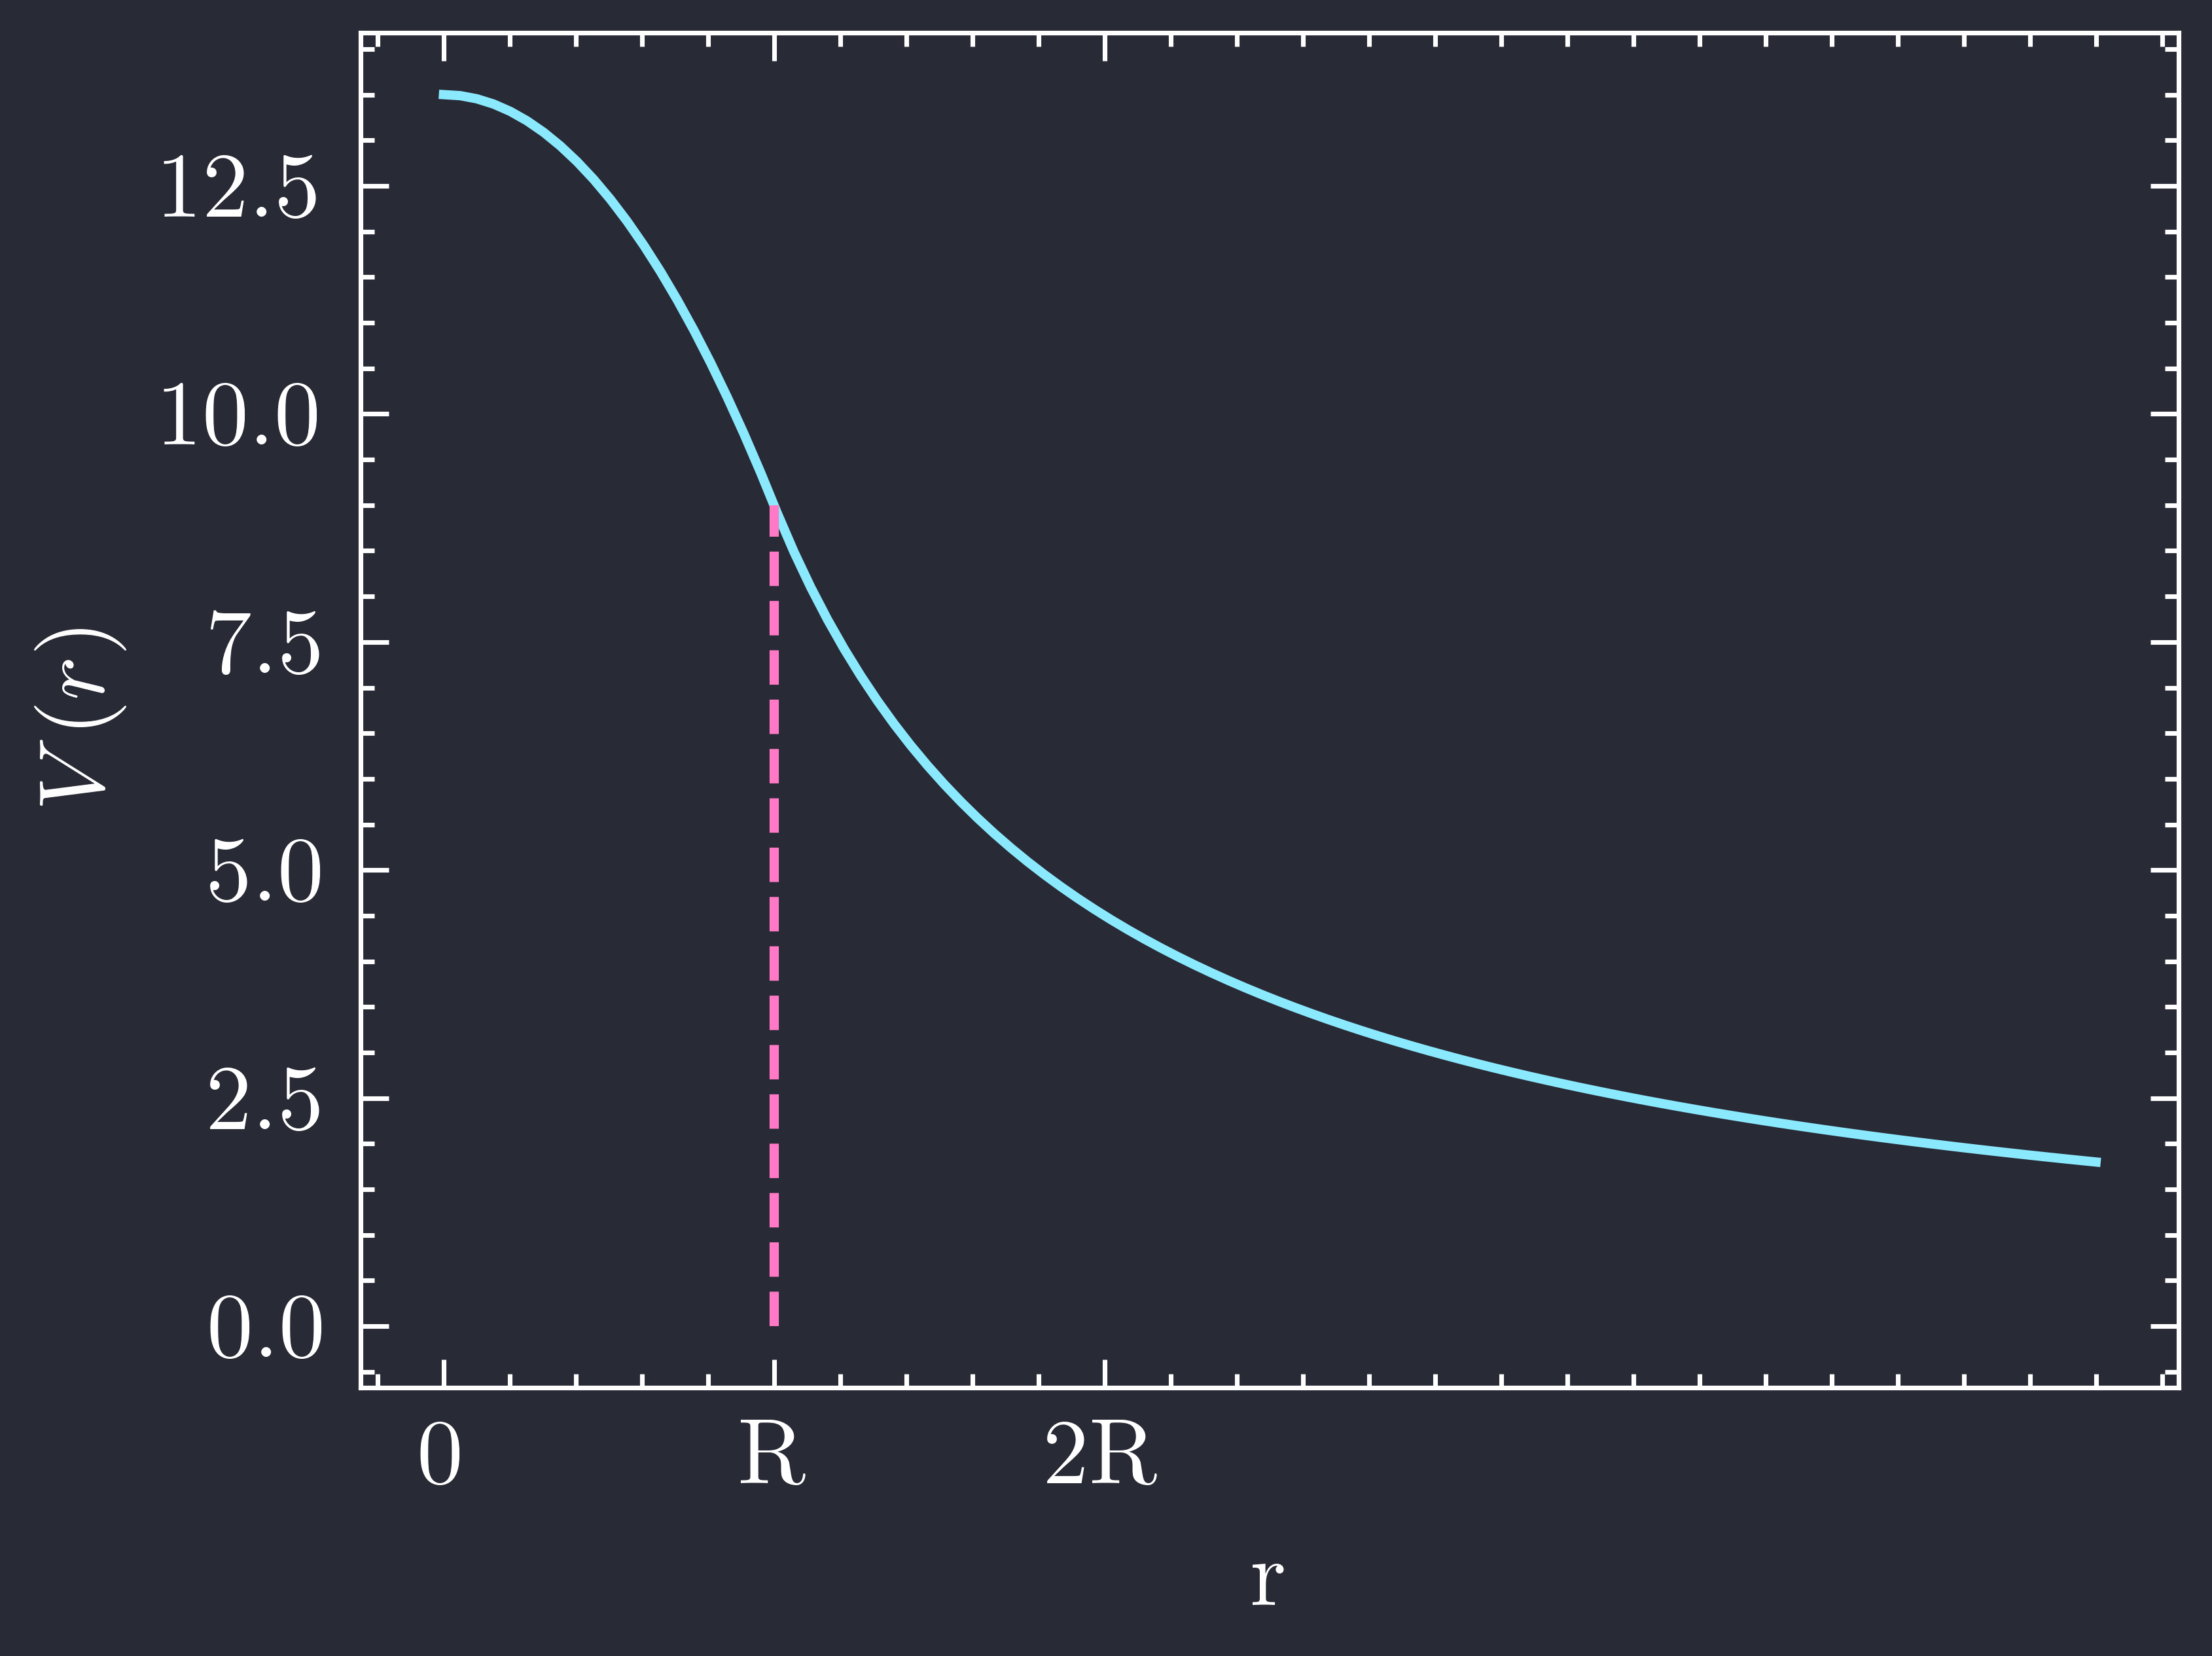
\includegraphics[width=0.5\linewidth]{images/fig2_21.png}
    \captionsetup{width=0.8\linewidth}
    \caption{Plot of $V(r)$ as a function of $r$ where $q = \qty{1}{nC}$ and $R = \qty{1}{m}$.}
    \label{fig:2_21}
\end{figure}

\newpage 
\paragraph{2.26} \label{prob:2_25}
From Griffiths % griffiths 2.27 + 2.30
\begin{align*} \tag{2.27} \label{eq:2_27}
    V(r) &= \ke \sum_{i = 1}^n \frac{q_i}{\scriptr_i}
\end{align*}
and
\begin{align*} \tag{2.30} \label{eq:2_30}
    V = \ke \int \frac{\lambda(\vb r')}{\scriptr} \dd{\ell'} \qand V = \ke \int \frac{\sigma(\vb r')}{\scriptr} \dd{a'} 
\end{align*}
\begin{enumerate}
    \item [(a.1)] Two point charges $+q$ a distance $d$ apart: Find the potential a distance $z$ above the center of the charges:
    \begin{figure*}[ht]
        \centering
        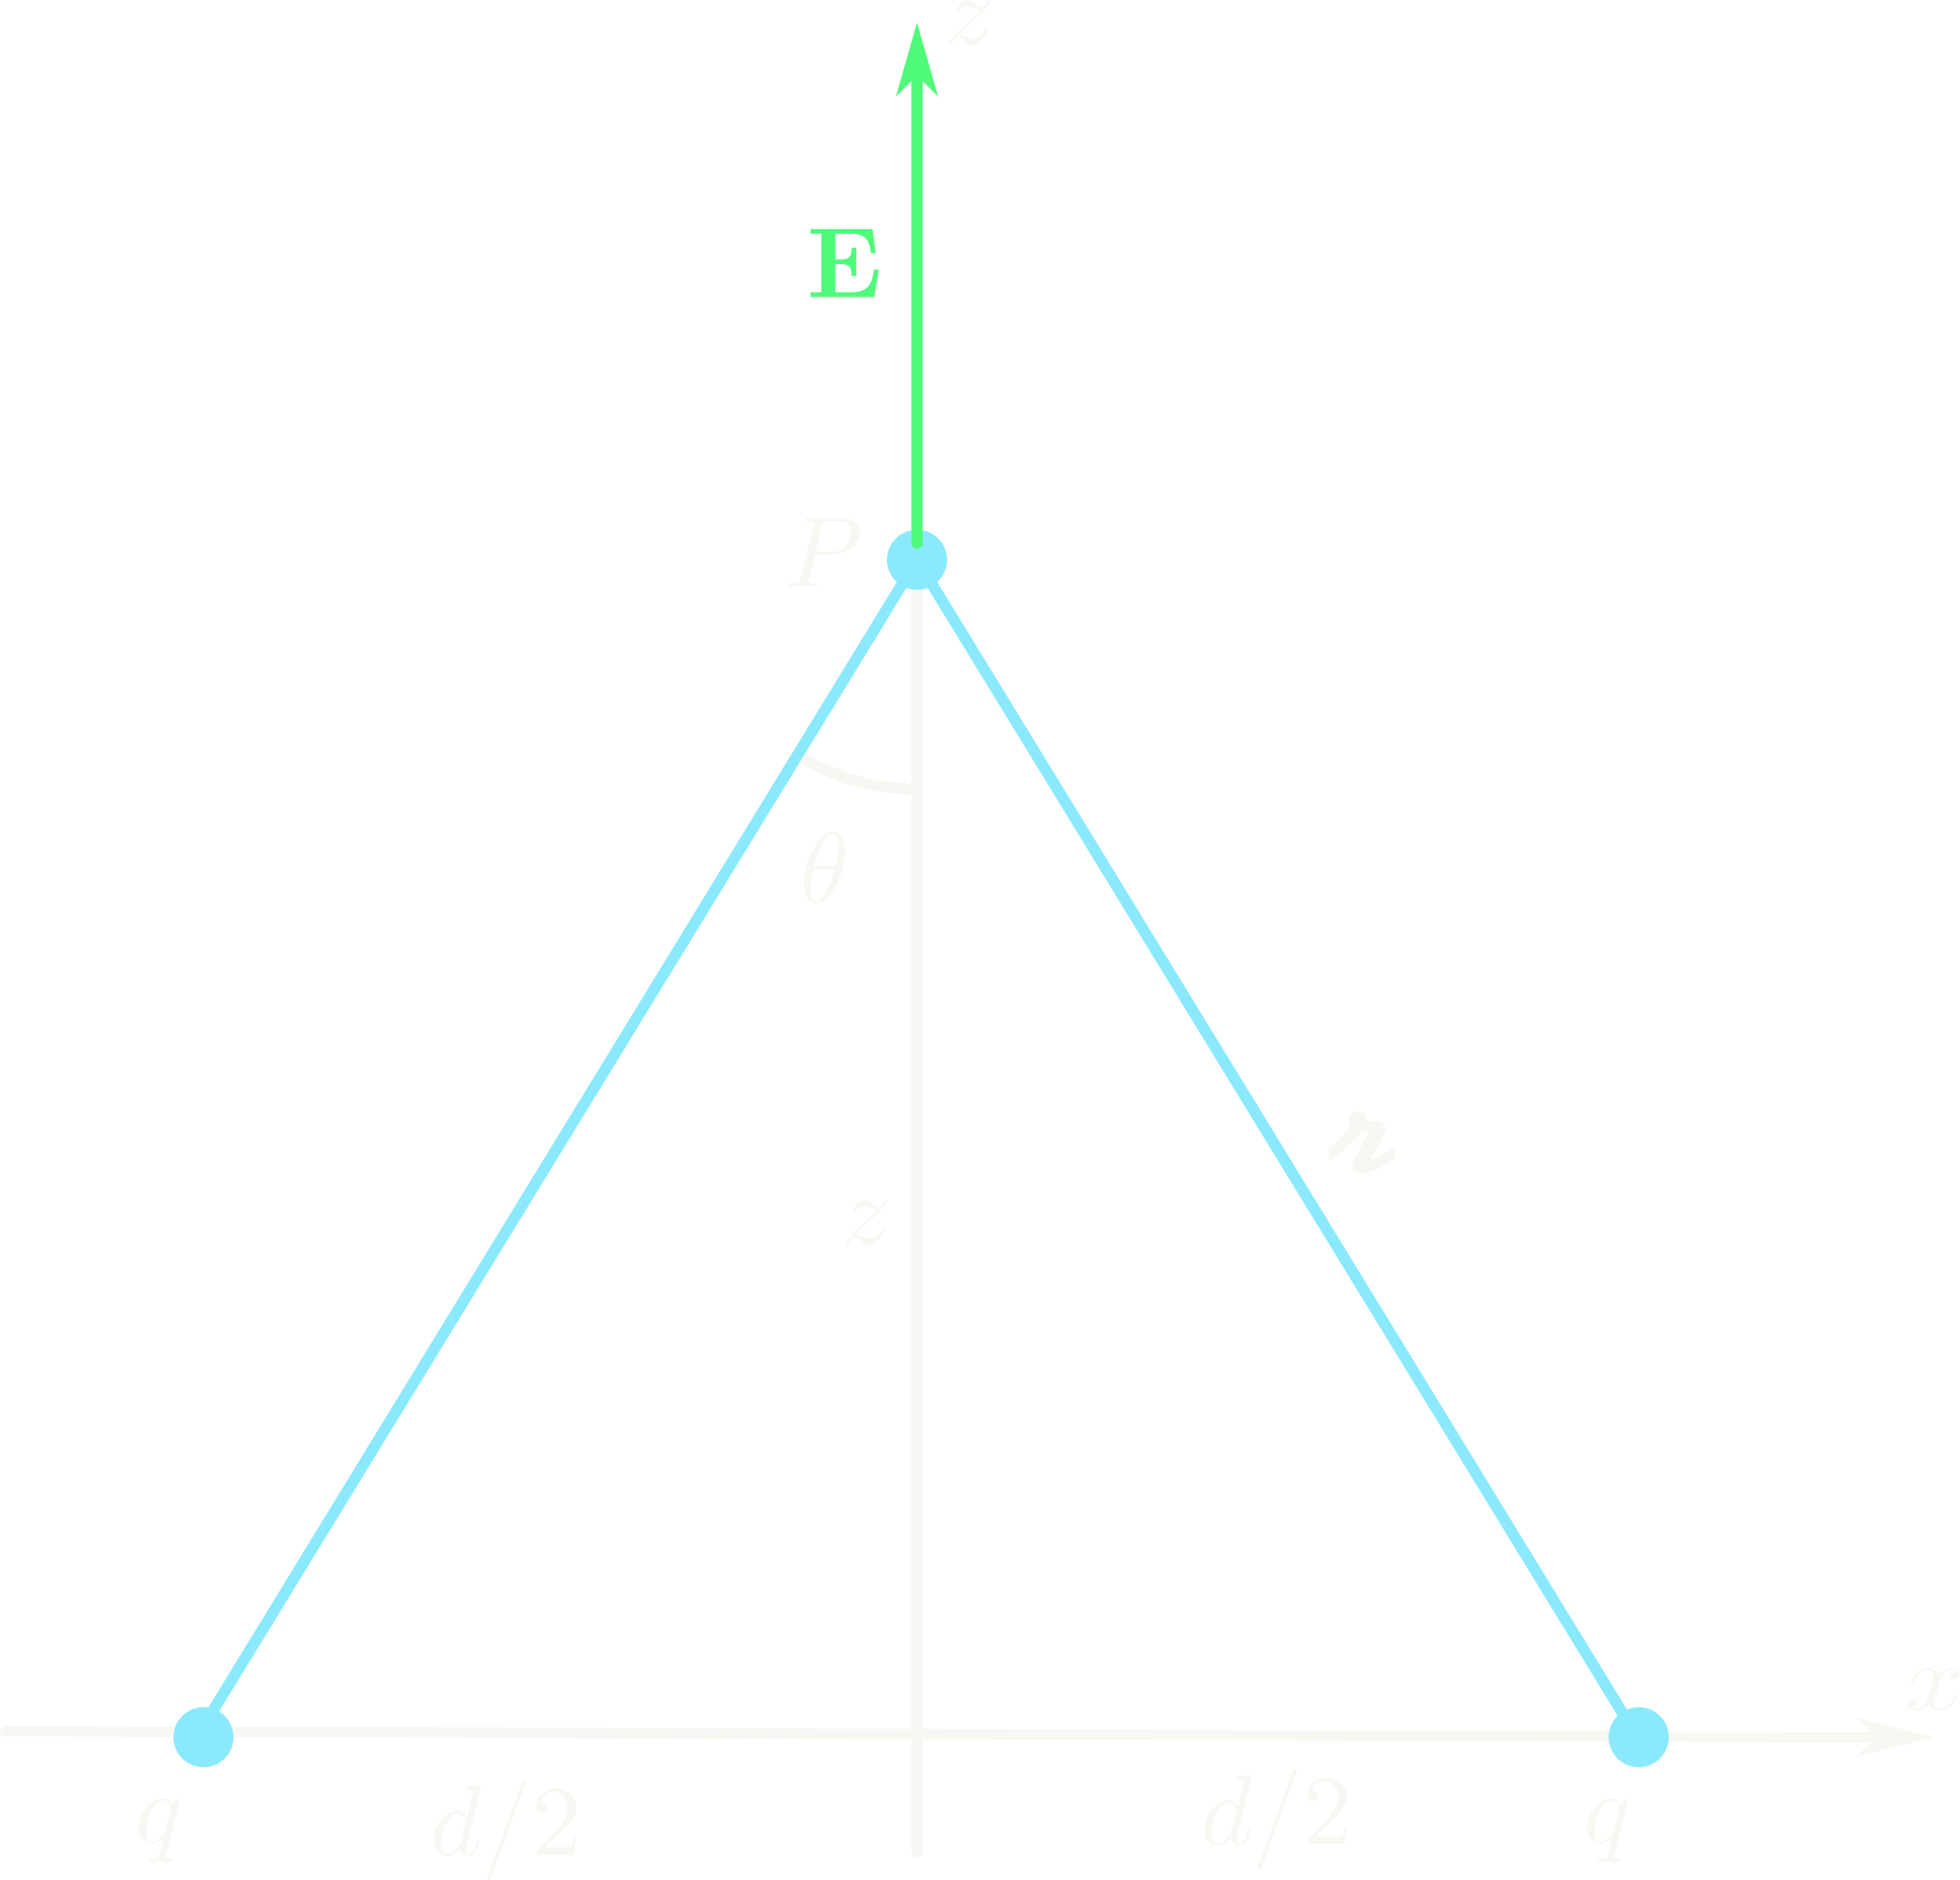
\includegraphics[width=0.5\linewidth]{images/hw2_25a.png}
        \captionsetup{width=0.8\linewidth}
        \caption{Two point charges $+q$ a distance $d$ apart.}
        \label{fig:2_25a}
    \end{figure*}
    Using Eq. \eqref{eq:2_27}, the potential is
    \begin{align*}
        &V_a = \ke \qt(\frac{q}{\sqrt{z^2 + \frac{d^2}{4}}} + \frac{q}{\sqrt{z^2 + \frac{d^2}{4}}}) \\
        &\boxed{V_a = \ke \frac{2q}{\sqrt{z^2 + \frac{d^2}{4}}}}
    \end{align*}
    \item [(a.2)] Computing the electric field $\vb E = -\grad V$:
    \begin{align*}
        \vb E_a &= -\pdv{V_a}{z} \vu z \\
        &= -\ke \frac{-1}{2} \frac{2q(2z)}{\qt(z^2 + \frac{d^2}{4})^{3/2}} \vu z
    \end{align*}
    simplifying to
    \begin{align*}
        \boxed{\vb E_a = \ke \frac{2qz}{\qt(z^2 + \frac{d^2}{4})^{3/2}} \vu z}
    \end{align*}
    which is the same as Ex. 2.1
    \begin{figure*}
        \centering
        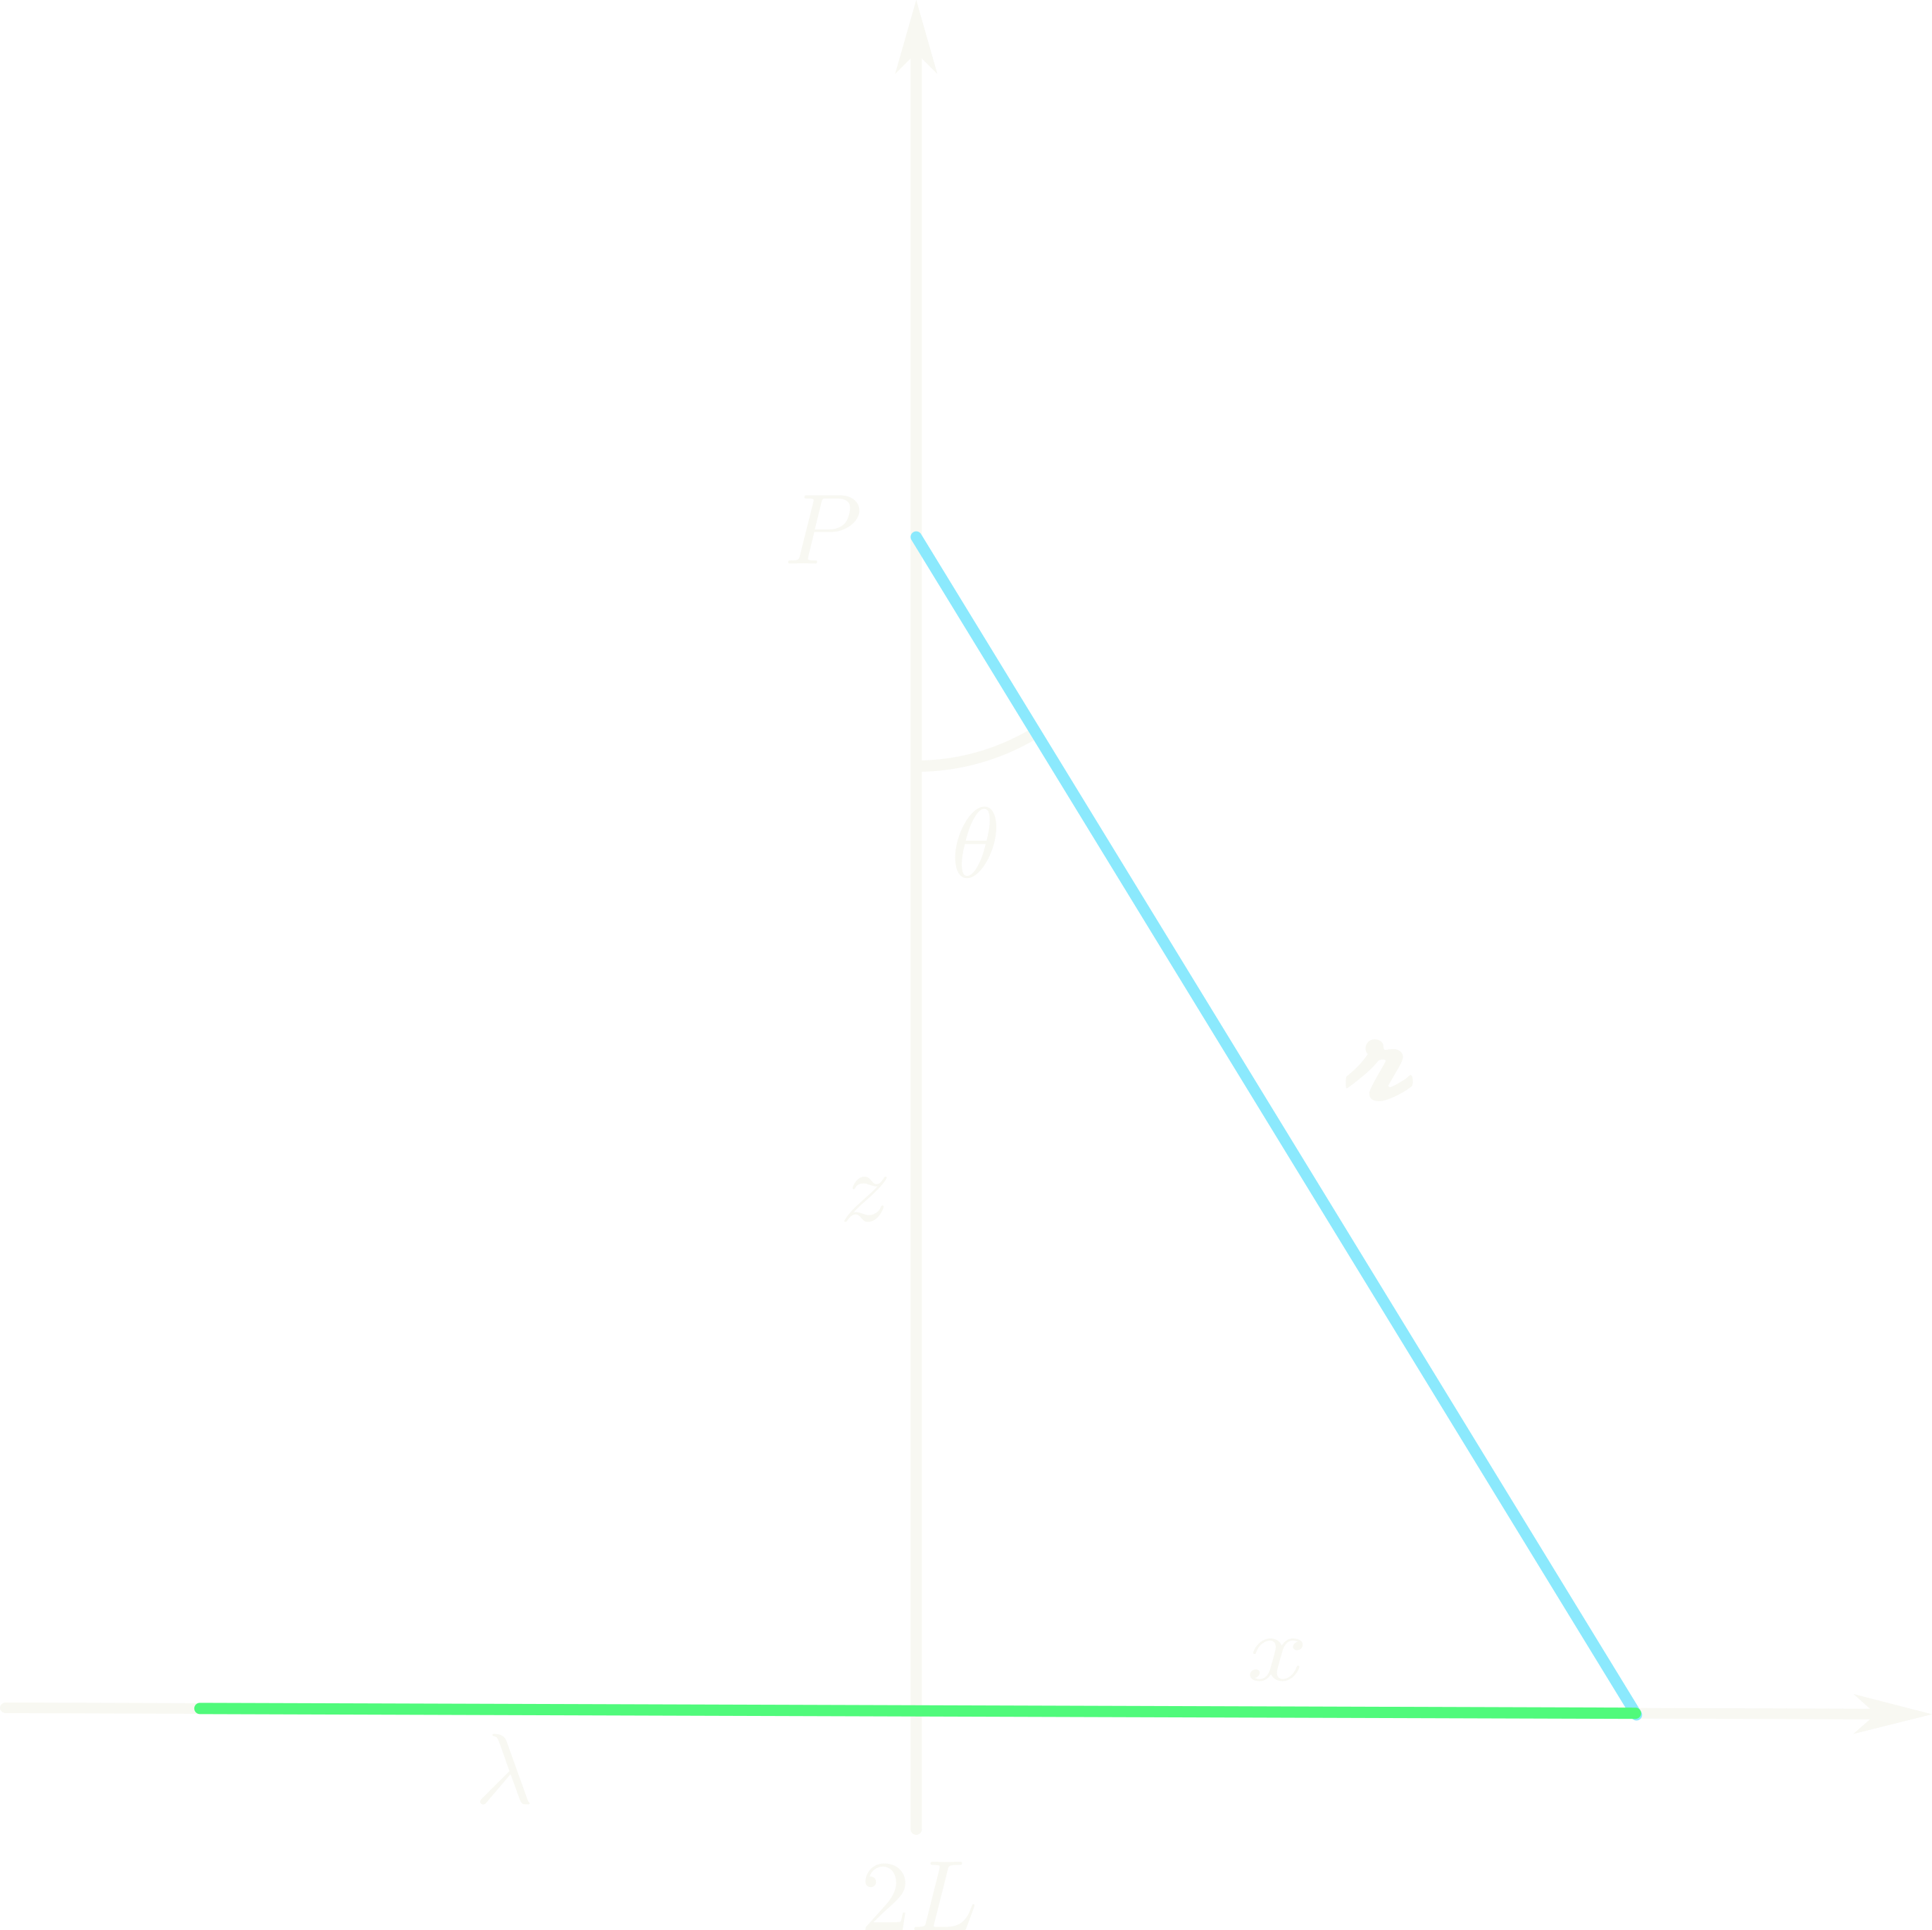
\includegraphics[width=0.5\linewidth]{images/hw2_25b.png}
        \captionsetup{width=0.8\linewidth}
        \caption{A line charge of density $\lambda$.}
        \label{fig:2_25b}
    \end{figure*}
    \item [(b.1)] Using Eq. \eqref{eq:2_30}, the potential is
    \begin{align*}
        V_b &= \ke \lambda \int_{-L}^L \frac{1}{\sqrt{z^2 + x^2}} \dd{x}
    \end{align*}
    To solve the integral, we can use the substitution from the trig identity
    \begin{align*}
        \cosh^2 u - \sinh^2 u &= 1 \\
        \implies z^2 \cosh^2 u &= z^2 + z^2\sinh^2 u \\
        &= z^2 + x^2
    \end{align*}
    where 
    \begin{align*}
        x &= z \sinh u \implies u = \arcsinh \frac{x}{z} \\
        \dd{x} &= z \cosh u \dd{u}
    \end{align*}
    Thus the integral becomes
    \begin{align*}
        V_b &= \ke \lambda \int \frac{\cancel{z \cosh u}}{\cancel{z \cosh u}} \dd{u} \\
        &= \ke \lambda u \eval_{-L}^L \\
        &= \ke \lambda \qt[\arcsinh{\frac{L}{z}} - \arcsinh{\frac{-L}{z}}]
    \end{align*}
    Using $\arcsinh \qt(a) = \ln \abs{a + \sqrt{a^2 + 1}}$:
    \begin{align*}
        \implies \arcsinh(\frac{L}{z}) &= \ln \abs{\frac{L}{z} + \sqrt{\qt(\frac{L}{z})^2 + 1}} \\
        &= \ln \abs{\frac{1}{z}(L + \sqrt{L^2 + z^2})}
    \end{align*}
    so the potential is
    \begin{align*}
        \boxed{V_b = \ke \lambda \ln \abs{\frac{L + \sqrt{L^2 + z^2}}{-L + \sqrt{L^2 + z^2}}}}
    \end{align*}
    \item[(b.2)] The electric field is
    \begin{align*}
        \vb E_b &= -\pdv{V_b}{z} \vu z \\
        &= -\ke \lambda \qt[ \frac{1}{L + \sqrt{L^2 + z^2}} \qt(\frac{1}{2} \frac{2z}{\sqrt{L^2 + z^2}})
            - \frac{1}{-L + \sqrt{L^2 + z^2}} \qt(\frac{1}{2} \frac{2z}{\sqrt{L^2 + z^2}})]\vu z \\
        &= -\ke \lambda \frac{z}{\sqrt{L^2 + z^2}} \qt[\frac{-L + \sqrt{L^2 + z^2}}{-L^2 + (L^2 + z^2)} - \frac{L + \sqrt{L^2 + z^2}}{-L^2 + (L^2 + z^2)}] \vu z \\
        &= -\ke \lambda \frac{-2Lz}{z^2 \sqrt{L^2 + z^2}} \vu z
    \end{align*}
    simplifying to
    \begin{align*}
        \boxed{\vb E_b = \ke \frac{2\lambda L}{z \sqrt{L^2 + z^2}} \vu z}
    \end{align*}
    which is the same as Ex. 2.2

    \item[(c.1)] Using Eq. \eqref{eq:2_30} and polar coordinates, the potential is
    \begin{align*}
        V_c &= \ke \sigma \int_0^{2\pi} \int_0^R \frac{1}{\sqrt{z^2 + r^2}} r \dd{r} \dd{\theta} \\
        &= \ke 2\pi \sigma \int_0^R \frac{r}{\sqrt{z^2 + r^2}} \dd{r}
    \end{align*}
    substituting $u = z^2 + r^2$; $\dd{u} = 2r \dd{r}$:
    \begin{align*}
        V_c &= \ke \pi \sigma \int \frac{1}{\sqrt{u}} \dd{u} \\
        &= \ke \pi \sigma 2 \sqrt{z^2 + r^2} \eval_0^{R}
    \end{align*}
    thus
    \begin{align*}
        \boxed{V_c = \frac{\sigma}{2\epsilon_0} \qt[\sqrt{z^2 + R^2} - z]}
    \end{align*}
    \item[(c.2)] The electric field is
    \begin{align*}
        \vb E_c &= -\pdv{V_c}{z} \vu z \\
        &= -\frac{\sigma}{2\epsilon} \qt[\frac{z}{\sqrt{z^2 + R^2}} - 1] \vu z
    \end{align*}
    thus
    \begin{align*}
        \boxed{\vb E_c = \frac{\sigma}{2\epsilon_0} \qt[1 - \frac{z}{\sqrt{z^2 + R^2}}] \vu z}
    \end{align*}
    which is the same as Problem 2.6:
    \paragraph{2.6}
The electric field is only in the $z$-direction where $\cos\theta = z/\scriptr$:
\begin{align*}
    \vb{E} &= \frac{1}{4\pi\epsilon_0}
        \int \frac{\sigma}{\scriptr^2} \cos\theta \vu{z} \dd{\vb{a}} \\
    &= \frac{1}{4\pi\epsilon_0}
        \int \frac{\sigma z}{(z^2 + r^2)^{3/2}} \vu{z} \dd{\vb{a}}
\end{align*}
Using polar coordinates: since $\dd{\vb{a}} = r \dd{r} \dd{\theta} $
\begin{align*}
    \vb{E} &= \frac{1}{4\pi\epsilon_0}
        \int_0^{2\pi} \int_0^R \frac{\sigma z}{(z^2 + r^2)^{3/2}} \vu{z} r \dd{r} \dd{\theta} \\
    &= \frac{1}{4\pi\epsilon_0}
        \sigma z (2\pi) \vu{z} \int_0^R \frac{r}{(z^2 + r^2)^{3/2}} \dd{r} \\
    &= \frac{\sigma}{2\epsilon_0} z \vu{z} \qt[
            -\frac{1}{\sqrt{z^2 + r^2}}
        ]_0^R \\
    &= \frac{\sigma}{2\epsilon_0} z  \qt[
            \frac{1}{z} -\frac{1}{\sqrt{z^2 + R^2}}
        ] \vu{z} \\
    \vb E &= \frac{\sigma}{2\epsilon_0} \qt[1 - \frac{1}{\sqrt{z^2 + R^2}}] \vu{z}
\end{align*}
    \item[(d)] if the right-hand charge of Fig. \ref{fig:2_25a} is replaced by a charge $-q$, the potential at $P$ using Eq. \eqref{eq:2_27} is
    \begin{align*}
        V_d = 0 \implies \vb E_d = 0
    \end{align*}
    which contradicts the result from Prob 2.2. This is because point $P$ does not give us any information about the electric field which points in the $x$-direction.
    In fact any reference point on the $z$-axis will give us the same result. 
\end{enumerate}

\begin{figure*}[ht]
    \centering
    \begin{minipage}[b]{0.3\linewidth}
        \centering
        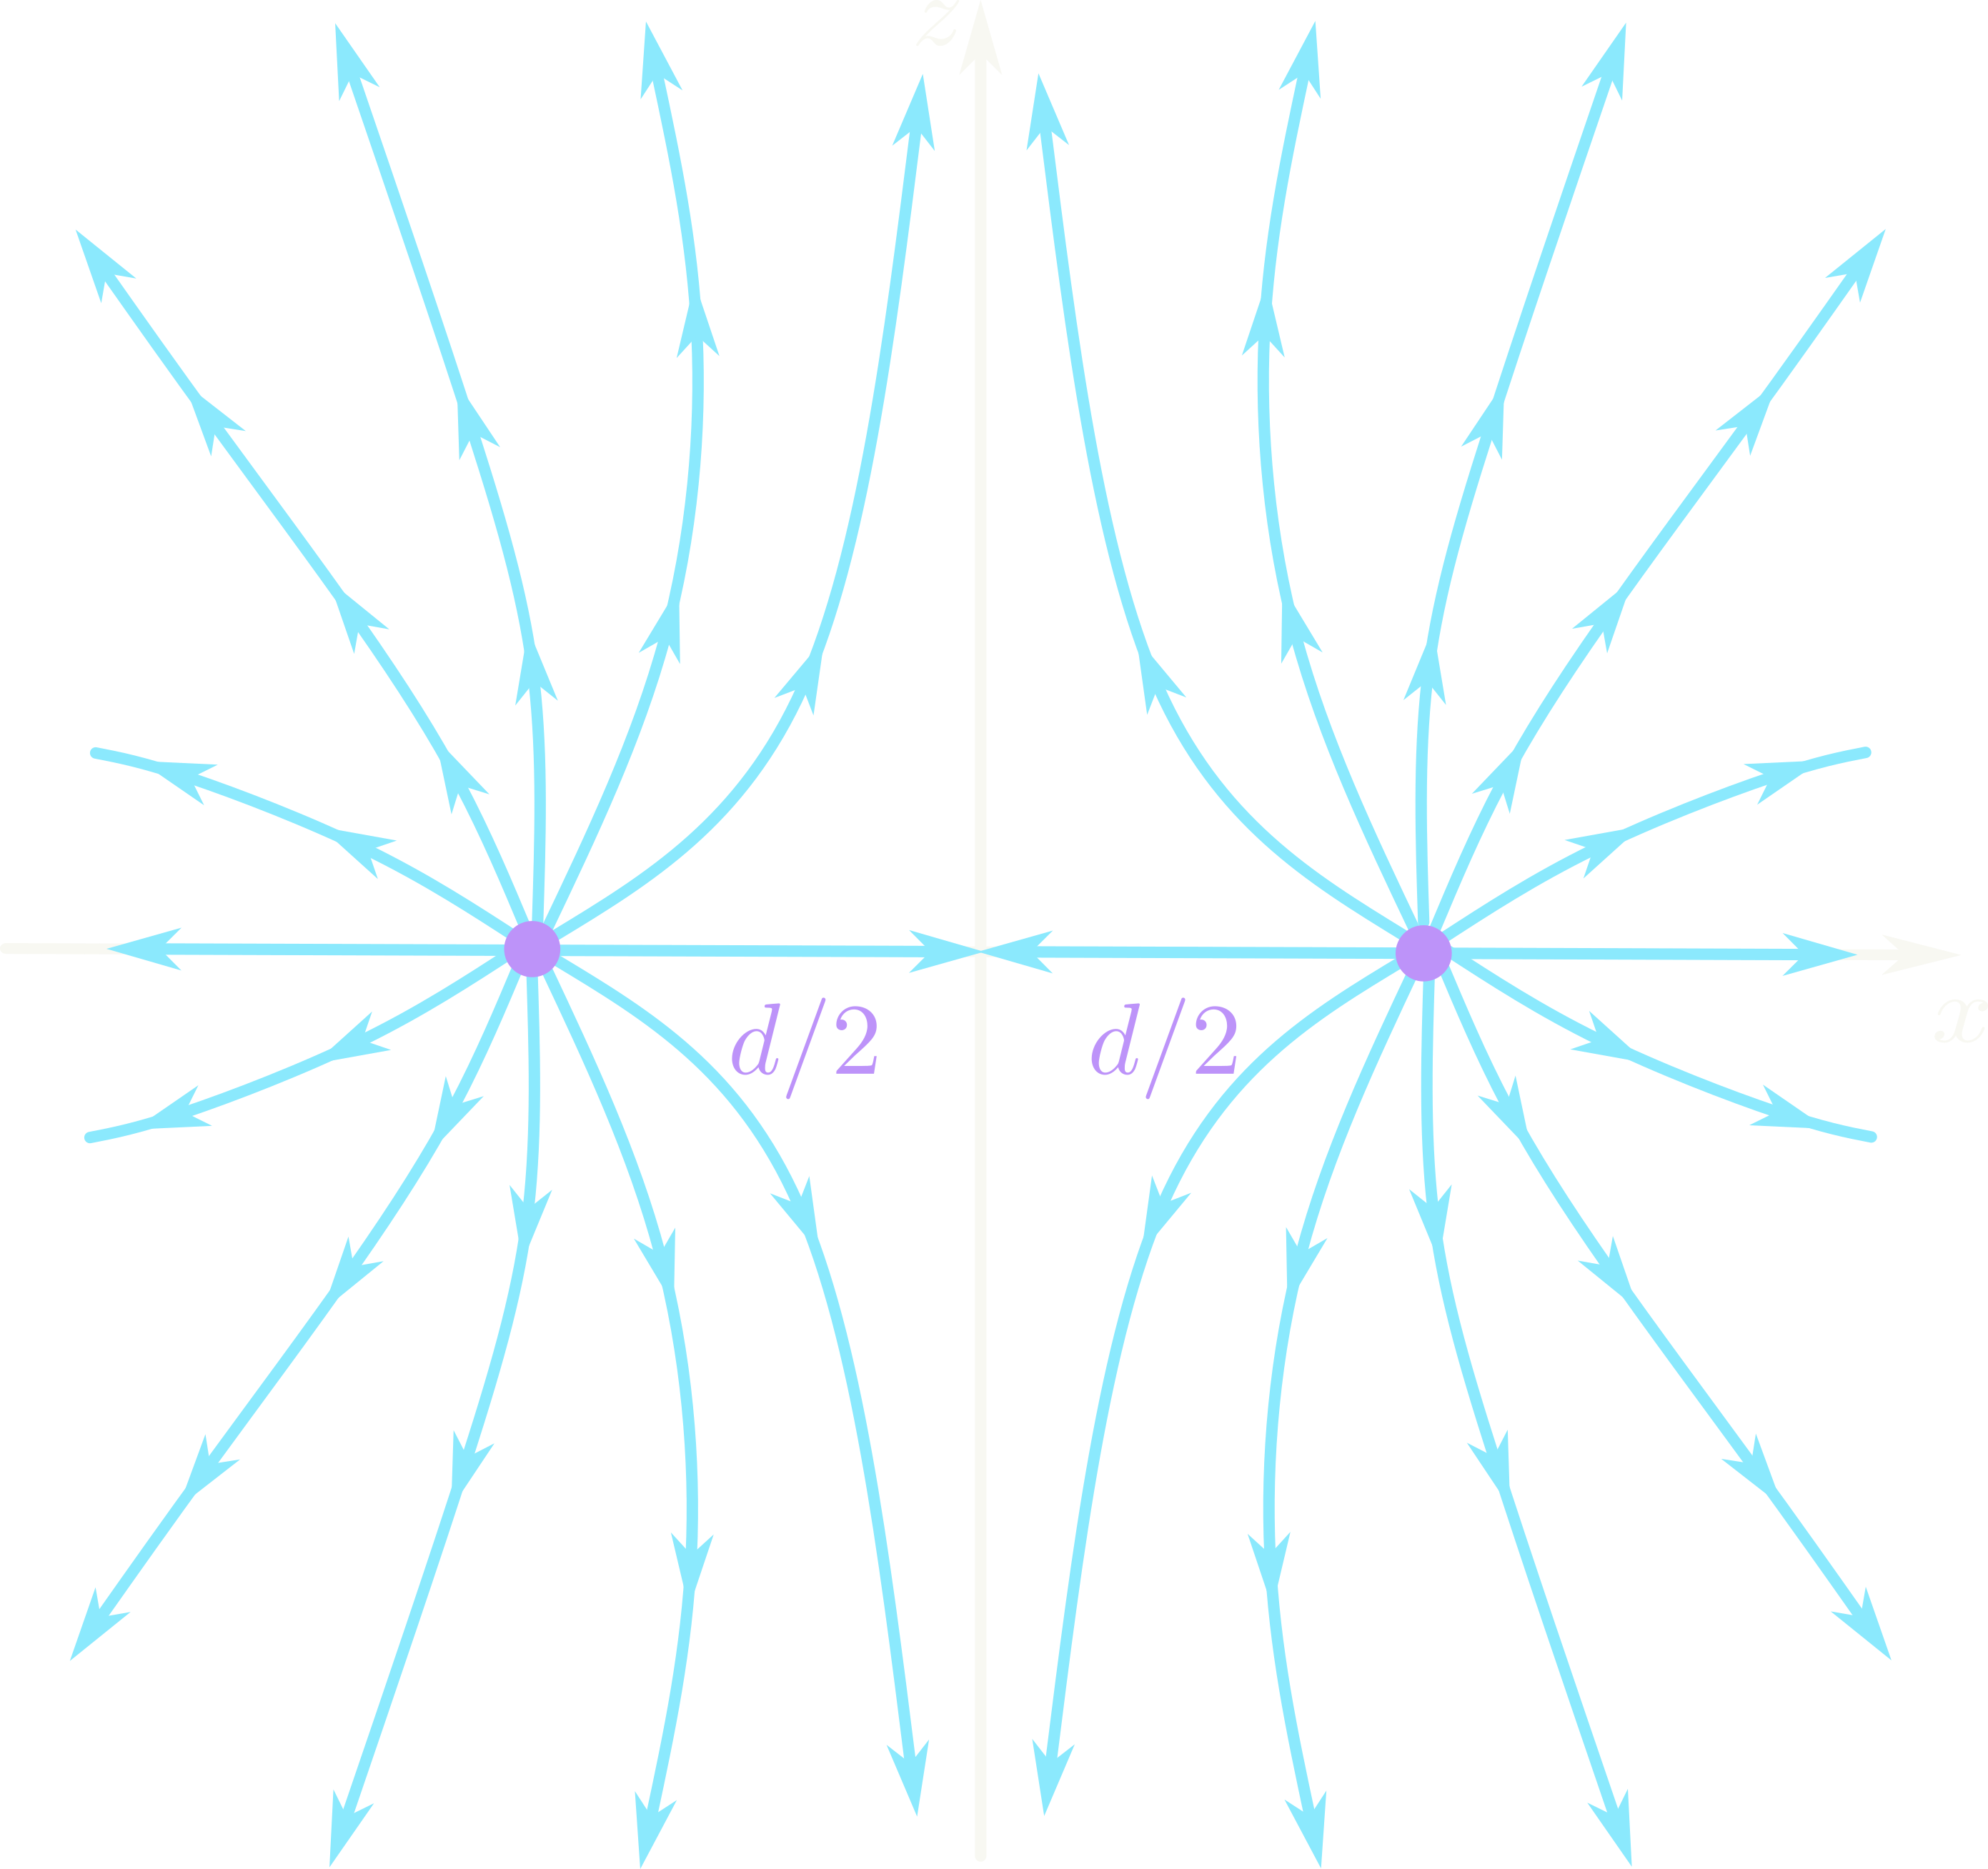
\includegraphics[width=\linewidth]{images/hw2_26a.png}
        \caption{E-field for (a)}
    \end{minipage}
    \hfill
    \begin{minipage}[b]{0.3\linewidth}
        \centering
        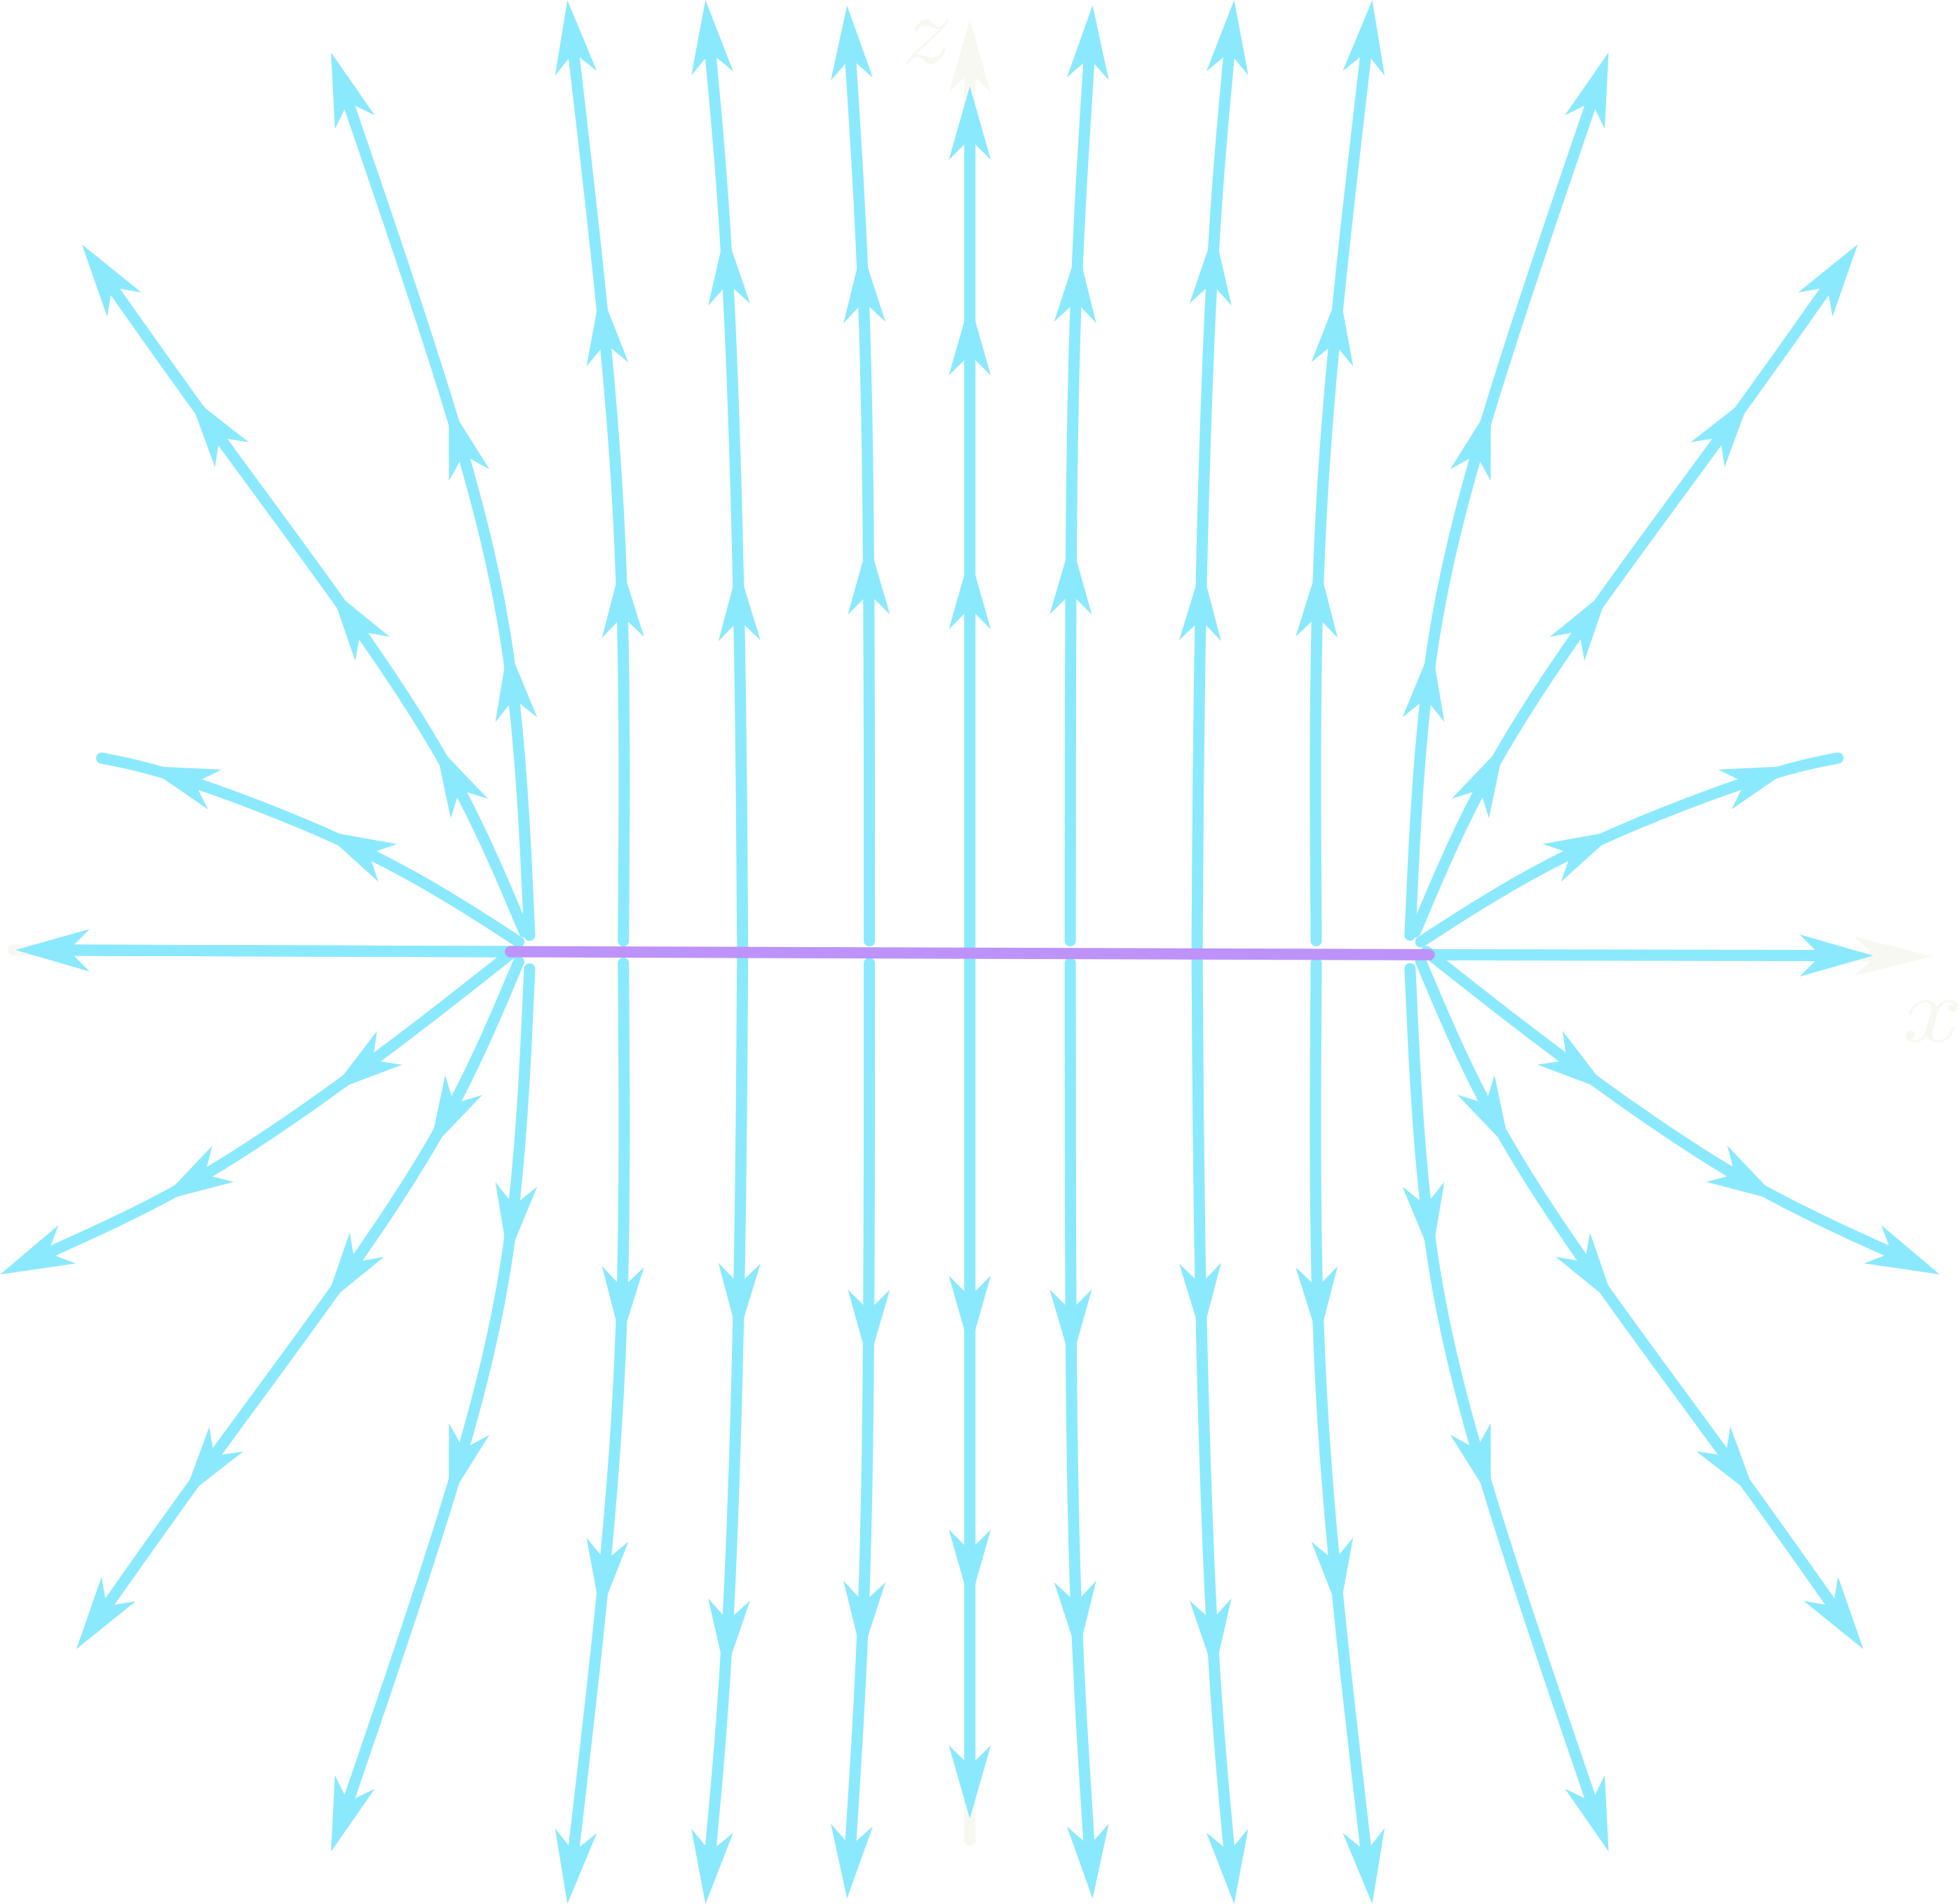
\includegraphics[width=\linewidth]{images/hw2_26b.png}
        \caption{E-field for (b)}
    \end{minipage}
    \hfill
    \begin{minipage}[b]{0.3\linewidth}
        \centering
        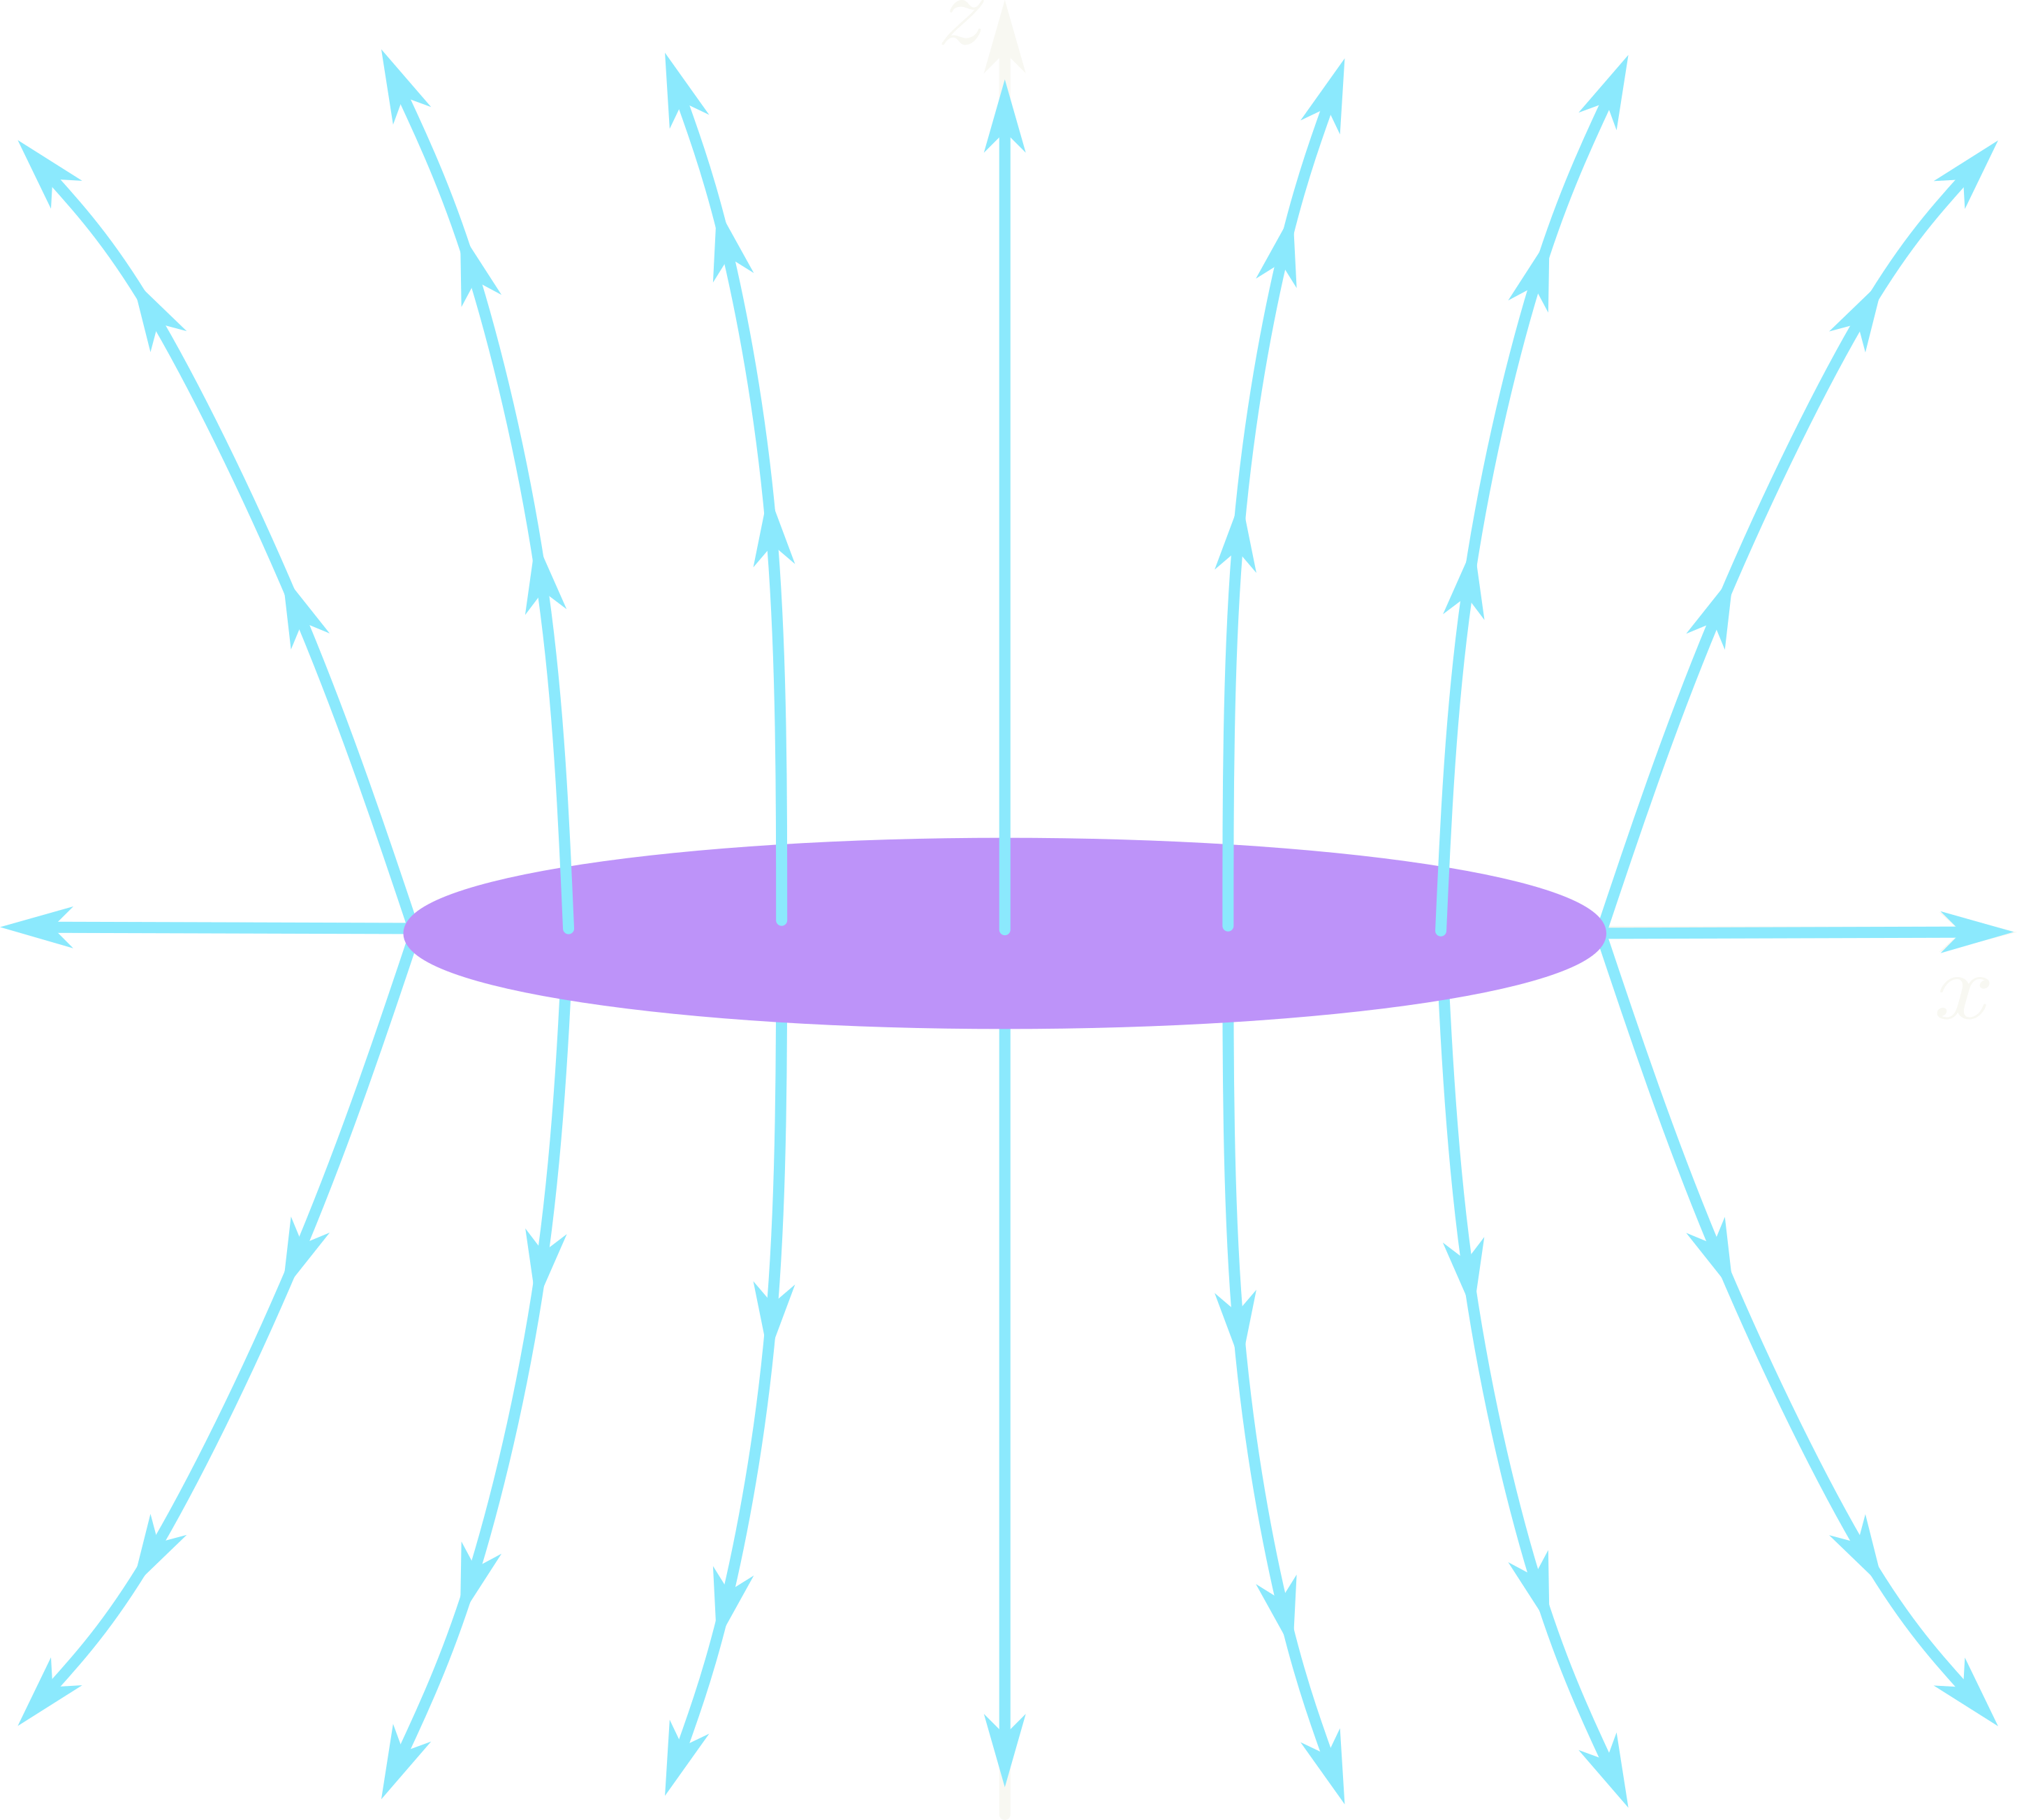
\includegraphics[width=\linewidth]{images/hw2_26c.png}
        \caption{E-field for (c)}
    \end{minipage}
\end{figure*}
\begin{figure*}[ht]
    \centering
    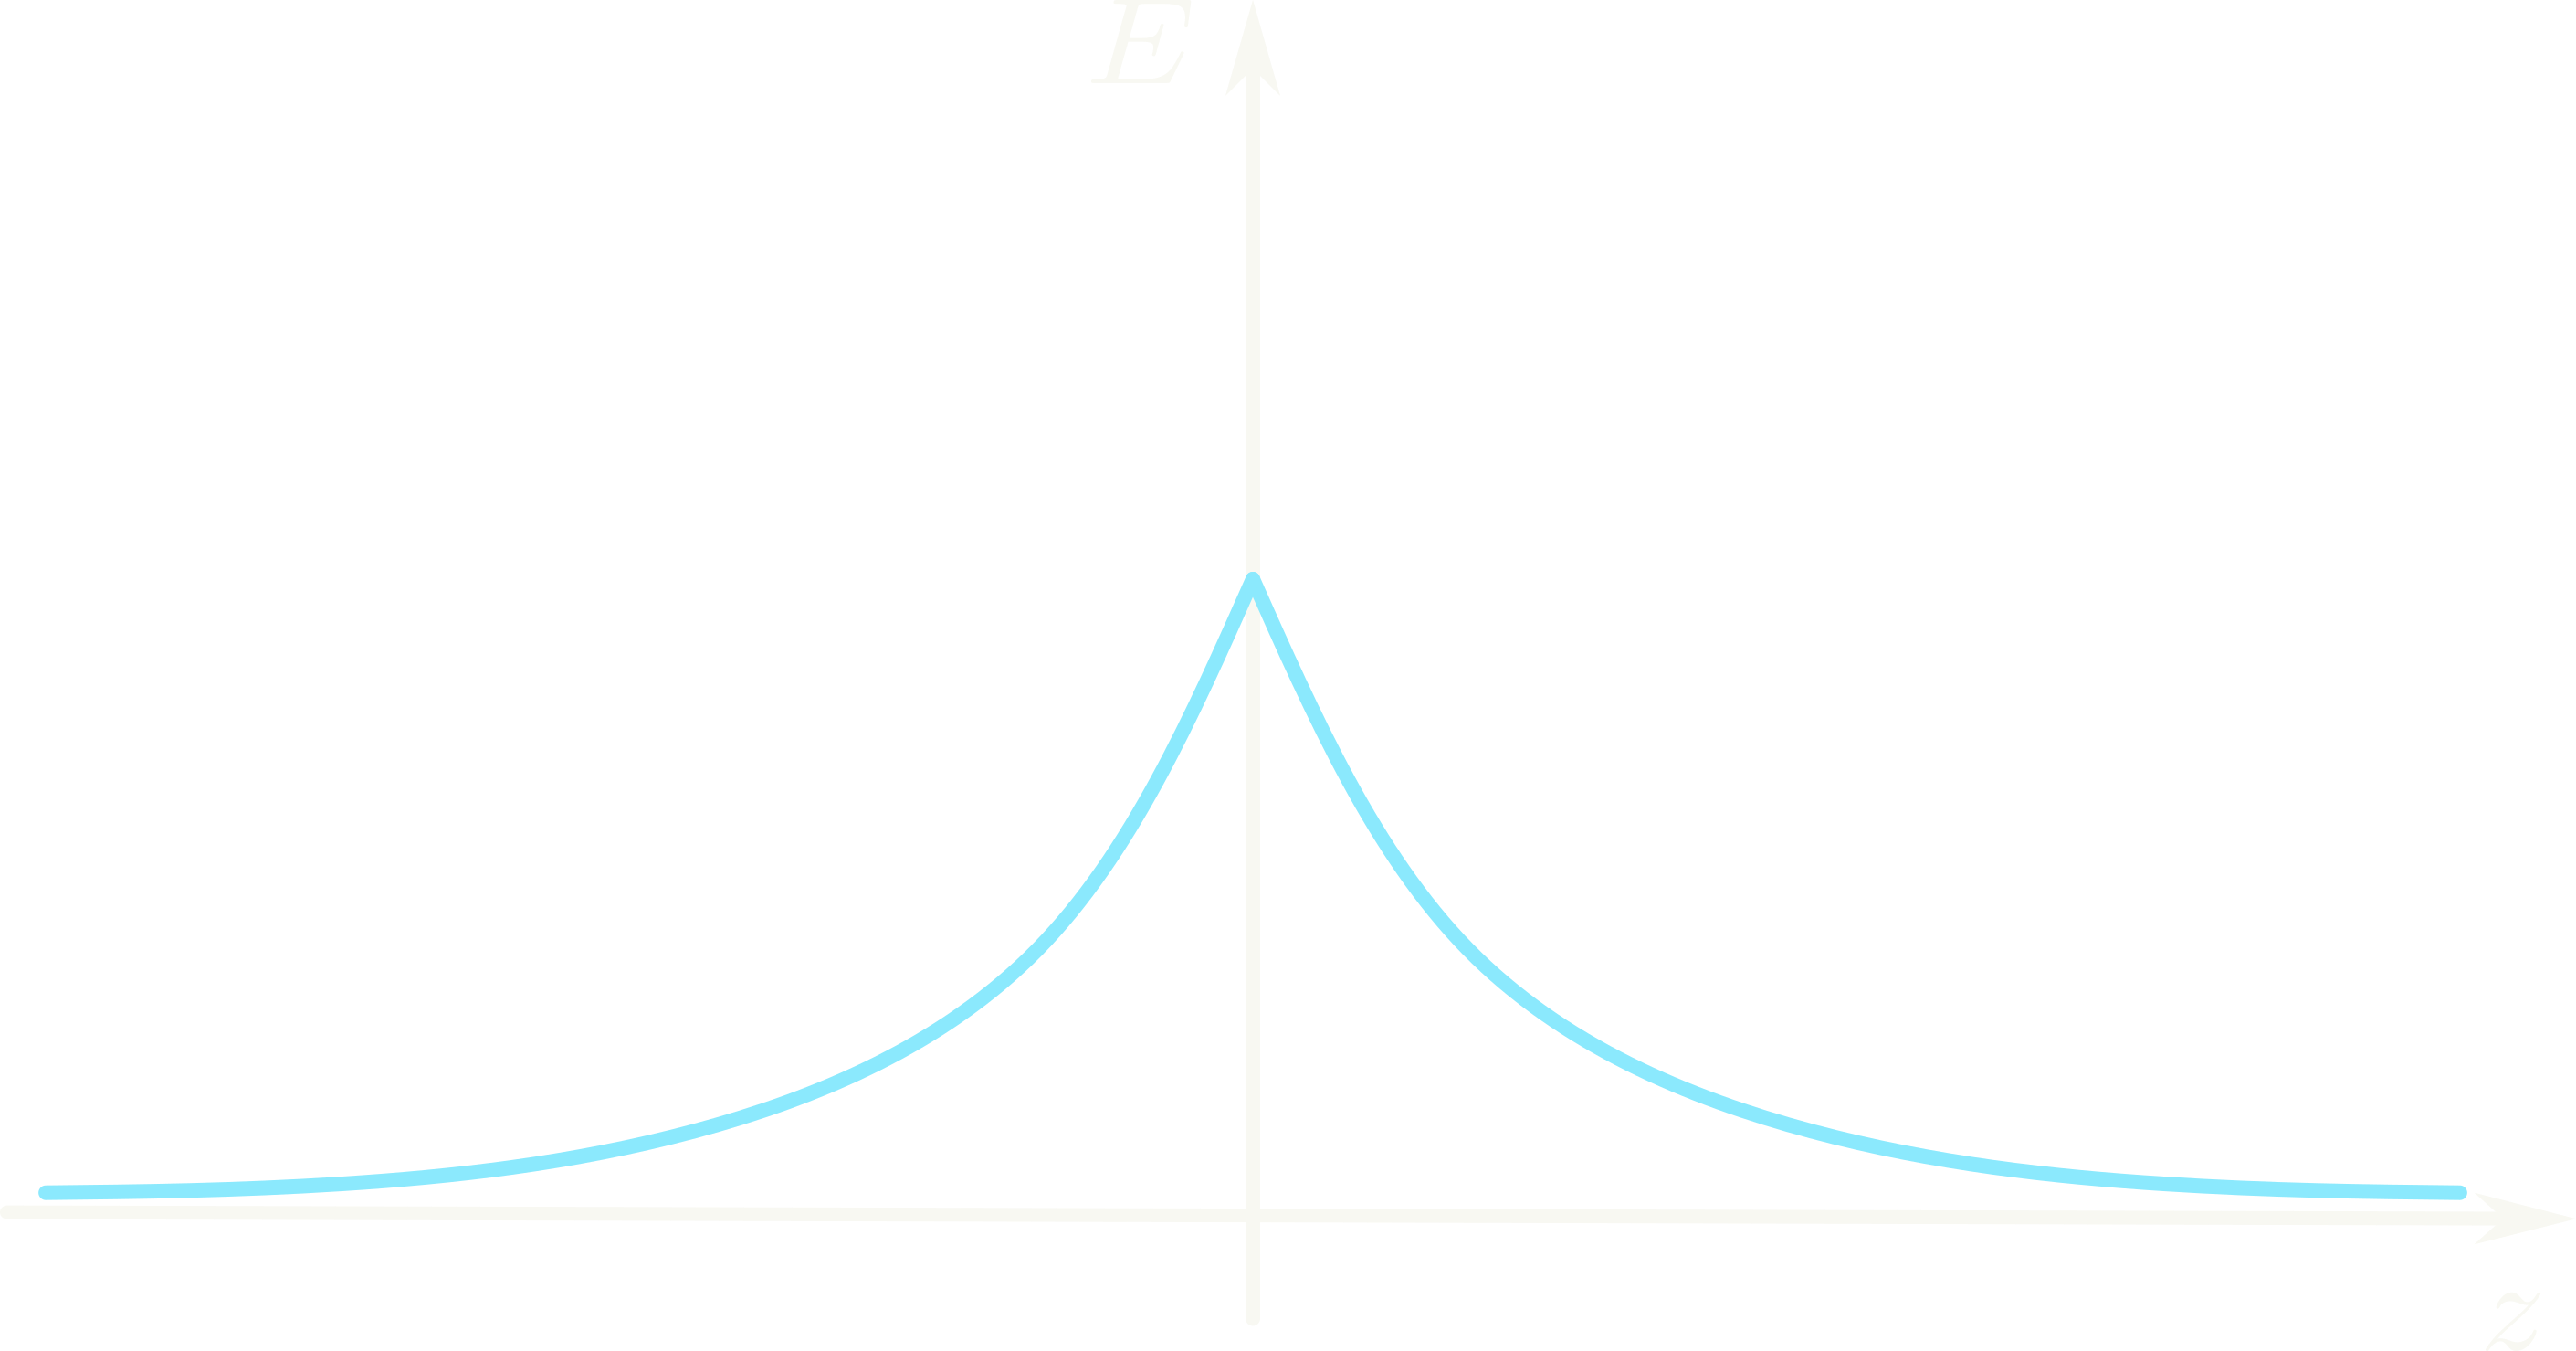
\includegraphics[width=0.3\linewidth]{images/hw2_26c2.png}
    \caption{E-field for (c) $E$ vs $z$}
\end{figure*}

\clearpage 
\newpage 
\paragraph{2.27}
\begin{figure}[ht]
    \centering
    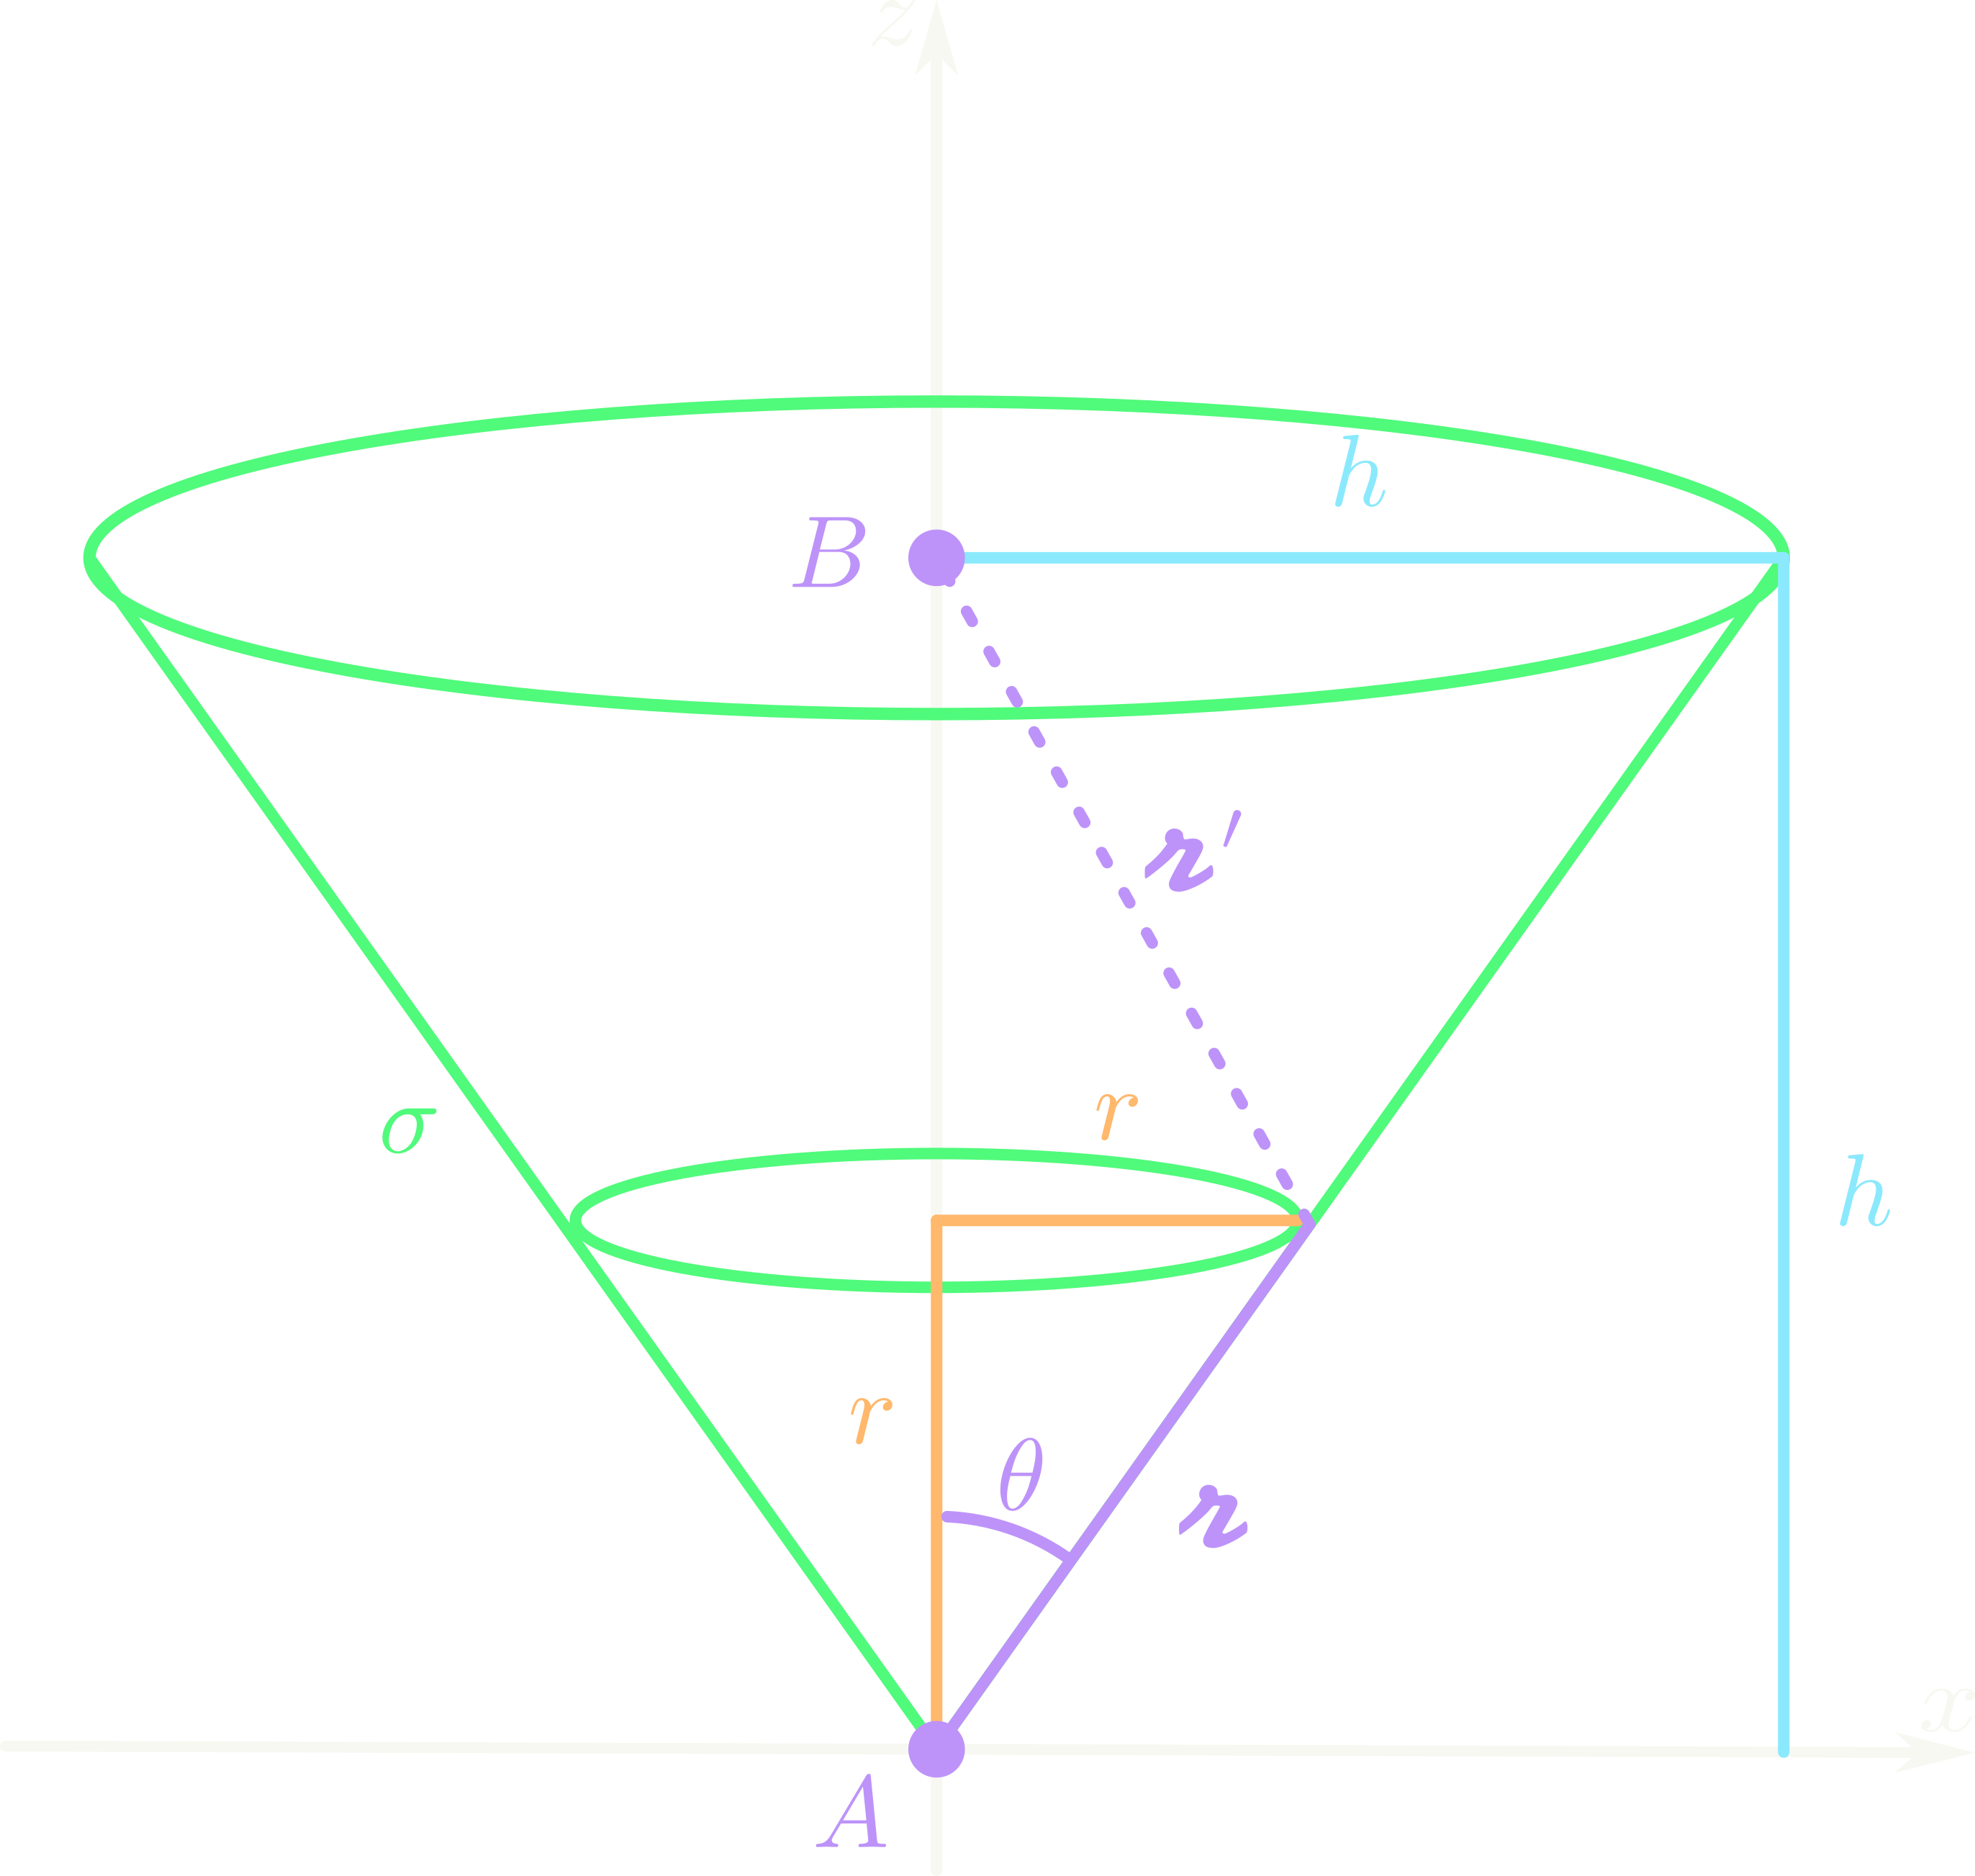
\includegraphics[width=0.5\linewidth]{images/hw2_26.png}
    \captionsetup{width=0.8\linewidth}
    \caption{Empty ice cream cone with surface charge density $\sigma$.}
    \label{fig:2_26}
\end{figure}
\begin{itemize}
    \item [(i)] Potential at $A$: Geometrically, we can see from the large right triangle that
    \begin{align*}
        \scriptr^2 = h^2 + h^2 \\
        \implies \scriptr = h\sqrt{2}, \quad h = \frac{\scriptr}{\sqrt{2}}
    \end{align*}
    and from the smaller right triangle
    \begin{align*}
        \scriptr^2 = 2r^2 \implies r = \frac{\scriptr}{\sqrt{2}}
    \end{align*}
    We can find the potential at $A$ using Eq. \eqref{eq:2_30} and integrate the rings of the cone along the slant length $0 \to h\sqrt{2}$
    which gives us the area element $\dd{a} = 2\pi r \dd{\scriptr}$:
    \begin{align*}
        V(A) &= \ke \int_0^{h\sqrt{2}} \frac{\sigma}{\scriptr} 2\pi r \dd{\scriptr} \\
        &= \frac{\sigma}{2\epsilon_0\sqrt{2}} \int_0^{h\sqrt{2}} \dd{\scriptr} \\
        &= \frac{\sigma}{2\epsilon_0\sqrt{2}} \scriptr \eval_0^{h\sqrt{2}} \\
        V(A) &= \frac{\sigma h}{2\epsilon_0}
    \end{align*}

    \item[(ii)] Potential at $B$: Using the law of cosines,
    \begin{align*}
        \scriptr'^2 = h^2 + \scriptr^2 - 2h\scriptr\cos\theta
    \end{align*}
    where
    \begin{align*}
        \cos\theta &= \frac{h}{\scriptr} \\
        &= \frac{h}{h\sqrt{2}} = \frac{1}{\sqrt{2}} = \frac{\sqrt{2}}{2} \\
        \implies \scriptr' &= \sqrt{h^2 + \scriptr^2 - h\scriptr\sqrt{2}}
    \end{align*}
    so the potential at $B$ is
    \begin{align*}
        V(B) &= \ke \int_0^{h\sqrt{2}} \frac{\sigma}{\scriptr'} 2\pi r \dd{\scriptr} \\
        &= \frac{\sigma}{2\epsilon_0\sqrt{2}} \int_0^{h\sqrt{2}} \frac{\scriptr}{\sqrt{h^2 + \scriptr^2 - h\scriptr\sqrt{2}}} \dd{\scriptr}
    \end{align*}
    I just used integral-calculator for this one\dots
    \begin{align*}
        V(B) &= \frac{\sigma}{2\epsilon_0\sqrt{2}} \qt[h\sqrt{2} \ln(1 + \sqrt{2})] \\
        V(B) &= \frac{\sigma h}{2\epsilon_0} \ln(1 + \sqrt{2})
    \end{align*}
    Finally the potential difference between $A$ and $B$ is
    \begin{align*}
        V(B) - V(A) = \frac{\sigma h}{2\epsilon_0} \ln(1 + \sqrt{2}) - \frac{\sigma h}{2\epsilon_0} \\
        \boxed{V(B) - V(A) = \frac{\sigma h}{2\epsilon_0} \qt[\ln(1 + \sqrt{2}) - 1]}
    \end{align*}
\end{itemize}

\newpage 
\paragraph{2.35} For a solid sphere radius $R$ and charge $q$
\begin{itemize}
    \item [(a)] From Problem \nameref{prob:2_21}
    \begin{align*}
        V = \ke \frac{q}{2R} \qt(3 - \frac{r^2}{R^2}) 
    \end{align*} and
    \begin{align*} \tag{2.43} \label{eq:2_43}
        W = \frac{1}{2} \int \rho V \dd{\tau}
    \end{align*}
    So the energy is 
    \begin{align*}
        W &= \frac{\rho}{2} \ke \frac{q}{2R} \int_0^{2\pi}\int_0^\pi\int_0^R \qt(3 - \frac{r^2}{R^2}) r^2 \sin\theta \dd{r} \dd{\theta} \dd{\phi} \\
        &= \frac{\rho}{2} \ke \frac{q}{2R} 4\pi \int_0^R \qt(3r^2 - \frac{r^4}{R^2}) \dd{r} \\
        &= \frac{\rho q}{4R\epsilon_0} \qt[r^3 - \frac{r^5}{5R^2}]_0^R \\
        &= \frac{\rho q}{4R\epsilon_0} \qt[R^3 - \frac{R^3}{5}] \\
        &= \frac{\rho q}{5\epsilon_0} R^2
    \end{align*}
    where the charge over the volume of the sphere is $\rho = \frac{q}{\frac{4}{3}\pi R^3}$, thus
    \begin{align*}
        W = \frac{q}{5\epsilon_0} R^2 \frac{q}{\frac{4}{3}\pi R^3} \\
        \boxed{W = \ke \frac{3q^2}{5R}}
    \end{align*}
    \item[(b)] Integrating over all space using 
    \begin{align*}\tag{2.45} \label{eq:2_45}
        W = \frac{\epsilon_0}{2} \int E^2 \dd{\tau}
    \end{align*}
    Where the electric field is
    \begin{align*}
        \vb{E}_{out} = \ke \frac{q}{r^2} \vu{r} \quad \vb{E}_{in} = \ke \frac{q}{R^3} r \vu{r}
    \end{align*}
    so the energy is
    \begin{align*}
        W &= \frac{\epsilon_0}{2} \frac{1}{(4\pi\epsilon_0)^2} 4\pi q^2 \qt[\int_0^R \frac{r^2}{R^6} r^2 \dd r + \int_R^\infty \frac{1}{r^4} r^2 \dd r] \\
        &= \ke \frac{q^2}{2} \qt[\int_0^R \frac{r^4}{R^6} \dd r + \int_R^\infty \frac{1}{r^2} \dd r] \\
        &= \ke \frac{q^2}{2} \qt[\frac{r^5}{5R^6}\eval_0^R - \frac{1}{R}\eval_R^\infty] \\
        &= \ke \frac{q^2}{2} \qt[\frac{R^5}{5R^6} + \frac{1}{R}] \\
        &= \ke \frac{q^2}{2} \frac{6}{5R} \\
        W &= \ke \frac{3q^2}{5R}
    \end{align*}
    checkmark.
    \item[(c)] For a spherical volume of radius $a$ and
    \begin{align*} \tag{2.44} \label{eq:2_44}
        W &= \frac{\epsilon_0}{2} \qt(\int_V E^2 \dd\tau + \oint_S V \vb E \cdot \dd\vb a)
    \end{align*}
    we can assume the volume is outside the charged sphere so
    \begin{align*}
        V &= \ke \frac{q}{r}
    \end{align*}
    From part (b), the first term is
    \begin{align*}
        \frac{\epsilon_0}{2} \int_V E^2 \dd\tau &= \ke \frac{q^2}{2} \qt[\frac{1}{5R} - \frac{1}{a} + \frac{1}{R}] \\
        &= \ke \frac{q^2}{2} \qt[\frac{6}{5R} - \frac{1}{a}]
    \end{align*}
    the second term is at $r = a$
    \begin{align*}
        \frac{\epsilon_0}{2} \oint_V V \vb E \cdot \dd\vb a &= \frac{\epsilon_0}{2} \frac{1}{(4\pi\epsilon_0)^2} \int \frac{q}{r} \frac{q}{r^2} r^2 \sin\theta \dd \theta \dd\phi \\
        &= \frac{4\pi\epsilon_0}{2} \frac{1}{(4\pi\epsilon_0)^2} \frac{1}{r} \eval_{r = a} \\
        &= \ke \frac{q^2}{2a}
    \end{align*}
    so the total energy is
    \begin{align*}
        W &= \ke \frac{q^2}{2} \qt[\frac{6}{5R} - \frac{1}{a}] + \ke \frac{q^2}{2a} \\
        &= \ke \frac{3q^2}{5R} 
    \end{align*}
    As $a \to \infty$ the $\int V\vb E \cdot \dd\vb a$ term goes to zero.
\end{itemize}

\newpage
\paragraph{2.40} Two cavities radii $a$ and $b$ in a conducting sphere of radius $R$ with a point charge $q_a$ and $q_b$ respectively in each cavity.
\begin{itemize}
    \item [(a)] Surface charge densities:
    
    On the surface of cavity $a$ the charge density is simply
    \begin{align*}
        \sigma_a = \frac{-q_a}{4\pi a^2}
    \end{align*}
    and 
    \begin{align*}
        \sigma_b = \frac{-q_b}{4\pi b^2}
    \end{align*}
    respectively. For the surface of the conducting sphere, the charge density is positive and equal to the superposition of the two charges:
    \begin{align*}
        \sigma_R = \frac{q_a + q_b}{4\pi R^2}
    \end{align*}
    \item [(b)] The field outside the conductor is equivalent to a point charge at the center of the sphere with the sum of the charges:
    \begin{align*}
        \vb E = \ke \frac{q_a + q_b}{r^2} \vu r
    \end{align*}
    \item [(c)] The field in cavity $a$ with respect to the center of the cavity is
    \begin{align*}
        \vb E_a = \ke \frac{q_a}{a^2} \vu a
    \end{align*}
    and in cavity $b$ is
    \begin{align*}
        \vb E_b = \ke \frac{q_b}{b^2} \vu b
    \end{align*}
    \item [(d)] The field due to to the cavity charge is zero in the exterior of the cavity, so there is no Force on $q_a$ or $q_b$.
    \item [(e)] If a charge $q_c$ was brought near the conductor from outside, there would be a change in (a) $\sigma_R$ and (b) $\vb E_{out}$.
\end{itemize}

\newpage
\paragraph{2.48} Net force of of the southern hemisphere extering on the northern hemisphere (solid sphere) with an inside Electric field (Problem 2.8)
\begin{align*}
    E_{in} = \ke \frac{Q}{R^3} \vb r 
\end{align*}
where the total force is 
\begin{align*}
    \vb F = Q \vb E = \ke \frac{Q^2}{R^3} \vb r
\end{align*}
Finding the net force exerted by the southern hemisphere: integrate $\dd F = \vb F / V$ over the southern hemisphere:
\begin{align*}
    \dd F &= \frac{1}{\frac{4}{3} \pi R^3} \ke \frac{Q^2}{R^3} \vb r \dd \tau \\
    &= \frac{3Q^2}{16\pi^2 \epsilon_0 R^6} \vb r \dd \tau
\end{align*}
The symmetry of the sphere implies that the Force is only in the $z$-direction i.e. $F_z = F \cos\theta$, so integrating over the southern hemisphere:
\begin{align*}
    \int_0^{2\pi} \int_0^{\pi/2} \int_0^R F_z \dd \tau &= \frac{3Q^2}{16\pi^2 \epsilon_0 R^6} \int_0^{2\pi} \int_0^{\pi/2} \int_0^R r \cos\theta r^2 \sin \theta \dd r \dd \theta \dd \phi \\
    &= \frac{3Q^2}{16\pi^2 \epsilon_0 R^6} (2\pi) \qt(\frac{r^4}{4})\eval_0^R \int_0^{\pi/2} \sin\theta \cos\theta \dd \theta \dd \phi \\
    &= \frac{3Q^2}{32\pi \epsilon_0 R^2} \frac{\sin^2 x}{2} \eval_0^{\pi/2} \\
    &= \boxed{\frac{3Q^2}{64\pi \epsilon_0 R^2}}
\end{align*}

\end{document}